\documentclass[12pt]{report}


%% Variables

\usepackage{ifthen}
\newboolean{coloured}
\setboolean{coloured}{false}
%\setboolean{coloured}{true}

%% Page structure and file output

\usepackage[screen, centering, right=1.5cm, top=1cm, includeall, includemp, reversemp]{geometry}
%\usepackage[screen, centering, includeall, includemp, reversemp]{geometry}

% limite les lignes orphelines et veuves
\widowpenalty=10000
\clubpenalty=10000
\raggedbottom


%% Text input, Fonts

\usepackage[utf8]{inputenc}
%\usepackage{ae,aeguill}
\usepackage{type1ec}%cm-super
\usepackage[T1]{fontenc}
\usepackage[T1]{tipa}
\let\ipa\textipa
\usepackage{vowel}
\newcommand{\BlankCell}{}


\usepackage{amssymb} % miscellaneous symbols

\newcommand{\allonge}{\textgreek{:}}

\renewcommand{\familydefault}{cmss}

%\renewcommand{\familydefault}{phv}


%% Floats (Graphics & Tables)

\usepackage{float}
\floatstyle{boxed} % ne marche pas avec seminar
\newfloat{exemple}{tbph}{loe}
\floatname{exemple}{Exemple}
\restylefloat{exemple} % \restylefloat*{exemple} prevents float from redefining the caption command (problems with seminar)

%\newfloat{exercice}{tbph}{loe}
%\floatname{exercice}{Exercice}
%\restylefloat{exercice} % \restylefloat*{exemple} prevents float from redefining the caption command (problems with seminar)


%\floatstyle{plain}
%\restylefloat{figure}
%\newfloat{figure}{H}{lof}
%\floatname{figure}{Figure}

%% \usepackage{caption2}
%% \newcommand*\mycaptionstyle{%
%%   \captionstyle{hang}%
%%   \renewcommand\captionfont{\small}%
%%   \renewcommand\captionlabelfont{\bfseries}%
%%   \setcaptionwidth{\textwidth}%
%%   \setcaptionmargin{-.05\textwidth}%\leftmargini
%%   \setlength{\abovecaptionskip}{0pt}%
%%   \setlength{\belowcaptionskip}{5pt}%
%%   \renewcommand\captionlabeldelim{ :}%
%%   \onelinecaptionstrue%
%% }
%% \mycaptionstyle


\usepackage{array,booktabs}
\newcolumntype{t}{>{\centering\slshape}p{.65\textwidth}}
\newcolumntype{d}{>{\centering\ttfamily}p{.20\textwidth}}
\newcolumntype{a}{>{\centering\ttfamily}p{.20\textwidth}}

\usepackage{multirow}
\usepackage{tabularx}
\usepackage{longtable}

%% Graphics and Colors

\usepackage{pstricks}

\usepackage[dvips]{graphicx}

\definecolor{SunBlue}{rgb}{.3,.3,.52}
\definecolor{SunBlueLight}{rgb}{.65,.65,.87}
\definecolor{SunBlueExtraLight}{rgb}{.75,.75,.97}
\definecolor{SunBlueDark}{rgb}{.45,.45,.67}
\definecolor{DarkOrange}{rgb}{1,.5,0}

\definecolor{Gray}{gray}{.5}
\definecolor{GrayLight}{gray}{.7}
\definecolor{GrayDark}{gray}{.3}

\definecolor{essai}{cmyk}{.1,.1,.1,.15}
\definecolor{hotpink}{rgb}{1,.43,.71}
\definecolor{DarkRed}{rgb}{.80,.10,.10}


\ifthenelse{\boolean{coloured}}{%
  \newcommand{\BGColor}{SunBlue}
  \newcommand{\FGColor}{white}
  \newcommand{\EMColor}{DarkOrange}
  \renewcommand{\emph}{\textcolor{\EMColor}}
  \newcommand{\BGColorLight}{SunBlueLight}
  \newcommand{\BGColorExtraLight}{SunBlueExtraLight}
  \newcommand{\BGColorDark}{SunBlueDark}
  \newcommand{\LINKColor}{SunBlueExtraLight}
}{% Turn to B&W for paper printing and replace italics with underlined
  \newcommand{\BGColor}{white}
  \newcommand{\FGColor}{black}
%  \newcommand{\EMColor}{DarkOrange}
%  \renewcommand{\emph}{\textcolor{\EMColor}}
  \newcommand{\BGColorLight}{GrayLight}
  \newcommand{\BGColorExtraLight}{white}
  \newcommand{\BGColorDark}{GrayDark}
  \newcommand{\LINKColor}{GrayDark}
%  \usepackage{ulem}
}
\pagecolor{\BGColor}
\color{\FGColor}
\usepackage{url}

%% Sections, Environments, Headers, Footers...

\usepackage{sectsty}
\allsectionsfont{\mdseries\sffamily}
\partfont{\centering\bfseries\color{\BGColorDark}\thispagestyle{empty}}
\chapterfont{\raggedleft\bfseries\color{\BGColorDark}\thispagestyle{empty}}
\sectionfont{\newpage\raggedleft\huge\color{\BGColorDark}\mdseries\sffamily}
\subsectionfont{\Large\mdseries\sffamily\sectionrule{2ex}{0pt}{-1ex}{1pt}}
\subsubsectionfont{\large\mdseries\sffamily}

\usepackage{example} % formats LaTeX examples with corresponding code
\usepackage{boxedminipage} % minipage with frame


\usepackage{fancyhdr}
\pagestyle{fancy}
\fancyhf{}
\fancyfoot[L]{\vspace{-8pt} \tiny \ttfamily%
  \psset{unit=10pt}%
  \psline[linewidth=.05,linecolor=\BGColorLight,linearc=.05]{-}(-5,0)(3,0)(3.1,0.5)(3.2,0)(3.3,-0.5)(3.4,0)(3.5,1)(3.6,0)(3.7,-1)(3.8,0)(3.9,2)(4,0)(4.1,-1)(4.2,0)(4.3,1)(4.4,0)(4.5,-0.5)(4.6,0)(4.7,.5)(4.8,0)(5,0)(18.8,0)(19,-0.4)(55,-0.4)%
   \rput[bl](6.5,-0.75){%
     \textcolor{\BGColorDark}{\today}%
   }%
}
\renewcommand{\headrulewidth}{0pt}




\usepackage[dvips,%
bookmarks=true,%
bookmarksnumbered,%
plainpages=false,%
pdfpagelabels,%
pdffitwindow=true,%
pdfcenterwindow=true,%
colorlinks=true,%
linkcolor=\FGColor,%
menucolor=menucolor,%
urlcolor=\LINKColor,%\FGColor,%
pdfstartview=Fit,%
pdfview=Fit,%
pdfstartpage=1]{hyperref}
\usepackage{breakurl}

%\usepackage[side,ragged,flushmargin,hang]{footmisc}
\usepackage[flushmargin]{footmisc}
\renewcommand{\footnotesize}{\scriptsize}

\usepackage{xspace}

\newcommand{\ttest}[3]{\ensuremath{t(#1)=#2,#3}}
\newcommand{\anova}[4]{\ensuremath{F(#1,#2)=#3,#4}}
\newcommand{\anovas}[5][1]{\ensuremath{F_#1(#2,#3)=#4,#5}}
\newcommand{\BiBTeX}{\textsc{BIB}\TeX\xspace}


%\renewenvironment{itemize}{\vfill\begin{itemize}}{\end{itemize}\vfill}

%\usepackage[greek,english]{babel}
\usepackage[greek,english,french]{babel}
\frenchbsetup{ReduceListSpacing=true,CompactItemize=false}
%\FrenchItemizeSpacingfalse
%\FrenchListSpacingfalse
\usepackage{babelbib}
\input{babelbst}

\setlength{\parindent}{0cm}
\setlength{\parskip}{6pt}

% Bibliography
\usepackage{bibentry}
\usepackage{natbib}

\newenvironment{biblist}{\begin{quotation}\small\setlength{\parindent}{-1cm}\indent}{\end{quotation}}






%%% Local Variables: 
%%% mode: latex
%%% TeX-master: "recueil-initiation-LaTeX"
%%% End: 


\fancyfoot[R]{\vspace{-12pt} \textcolor{\BGColorDark}{%
    \tiny \ttfamily Méthodologie de l'informatique -- Initiation à \LaTeX{}
    %%-- \og Sciences du Langage -- Informatisation des Langues \fg
    -- \input{univ-year}
    -- [\thepage] \vspace{18pt}
  }
}


\title{\Huge Master 2 \og Sciences du Langage \fg -- parcours \og Informatisation des Langues \fg\\
  Méthodologie de l'informatique -- Initiation à \LaTeX}
\author{Olivier Crouzet}



%%% Local Variables: 
%%% mode: latex
%%% TeX-master: "M2-Initiation-LaTeX-couleur"
%%% End: 



\begin{document}
\sffamily
%% \begin{abstract}
%%   Initiation à l'usage de \LaTeX{} pour les étudiants de l'école doctorale \og
%%   Connaissance, Langages, Culture \fg.
%% \end{abstract}
\maketitle




\renewcommand{\labelitemi}{%
  \vspace*{12pt}%
  \psline[linewidth=.8pt,linecolor=\BGColorDark,framearc=.70,arrowinset=0]{->}(-9pt,6pt)(-6pt,3pt)(0pt,3pt)%
}
\renewcommand{\labelitemii}{%
  \psline[linewidth=.6pt,linecolor=\BGColorLight,framearc=.70,arrowinset=0]{->}(-9pt,6pt)(-6pt,3pt)(0pt,3pt)%
}
\renewcommand{\labelitemiii}{%
  \psline[linewidth=.6pt,linecolor=\BGColorLight]{-oo}(-6pt,3pt)(0pt,3pt)%
}

%\renewcommand{\chaptername}{Séance}

% Contrôle de la profondeur d'affichage pour la Table des Matières
\setcounter{tocdepth}{1}     % Profondeur maxi pour intégration dans la TdM
\setcounter{secnumdepth}{1}  % Profondeur maxi pour affichage numérotation


\nobibliography{latex}
\bibliographystyle{apaformat}
%\nobibliography{latex}
%\bibliographystyle{apalike}







%%% Local Variables: 
%%% mode: latex
%%% TeX-master: "ED-Initiation-LaTeX-couleur"
%%% End: 


\tableofcontents


%\part{Premier contact avec \LaTeX}


\chapter{Présentation de \LaTeX}
\begin{center}
\begin{minipage}[r]{0.5\linewidth}
  Présentation des caractéristiques de la rédaction de documents avec
  \LaTeX. Différences par rapport aux traitements de texte
  WYSIWYG. Sources d'information. Structuration de documents. Notions
  d'instruction et d'environnement.
  \end{minipage}
\end{center}



%%%%%%%%%%%%%%%%%%%%%%%%%%%%%%%%%%%%%%%%%%%%%%%%%%%%%%%%%%%%%%%%%%%%%%%%%%%

%% Finir Emacs, Caractères réservés.

%% Parler de la compatibilité descendante (tout document compilable avec une ancienne version est également compilable sans modification de la mise en page avec les versions ultérieures).

%% Afficher les extensions des fichiers sous Windows (Panneau de Conf°, Options des dossiers, Masquer les extensions (décocher).


%%%%%%%%%%%%%%%%%%%%%%%%%%%%%%%%%%%%%%%%%%%%%%%%%%%%%%%%%%%%%%%%%%%%%%%%%%%



%\section{Plan de la formation \LaTeX}

\begin{enumerate}
  
  %% 4h
\item Introduction
  \begin{enumerate}
  \item Présentation de \TeX\ \& \LaTeX
  \item Quelques sources d'information indispensables
  \item Comparaisons entre les différents systèmes disponibles
  \item Premiers pas avec \LaTeX
  \item Initiation à l'utilisation d'\emph{Emacs}
  \end{enumerate}
  
  %% 4h
\item Rédaction de documents avec \LaTeX\
  \begin{enumerate}
  \item \LaTeX\ et les caractères accentués
  \item \LaTeX, mise en page, typographie
  \item Les caractères spéciaux (caractères réservés)
  \item Les composants d'un document \LaTeX\ (classe de documents, extensions,
    options)
  \item La classe de documents \emph{article} : votre premier document avec
    \LaTeX
  \end{enumerate}

%\item Formats de fichiers à connaître (tex, dvi, ps, pdf)
%\item Création de documents imprimables~: dvips, ghostscript, pdflatex
  
% 6h
\item \LaTeX : Utilisation avancée
  \begin{enumerate}
  \item Comment créer un fichier PDF à partir d'un fichier \LaTeX
  \item Les flottants -- 1 : graphiques
    \begin{enumerate}
    \item Insérer une image
    \item Positionner automatiquement un graphique sur la page : la notion de
      \og flottant \fg
    \end{enumerate}
  \item Les flottants -- 2 : tableaux
    \begin{enumerate}
    \item Construire un tableau
    \item Les tableaux flottants
    \item Les tableaux avec saut de page
    \end{enumerate}
  \end{enumerate}


\item Les éléments importants lors de la rédaction d'un document

  \begin{enumerate}

  \item Les principaux environnements disponibles
    
  \item Renvois, Indexes, Tables de matières, Annexes
    
  \end{enumerate}

\item La gestion des références bibliographiques (\textsc{BIB}\TeX)
    
  \begin{enumerate}
  \item \LaTeX et \BiBTeX
  \item Créer un fichier \BiBTeX : une base de données bibliographiques
  \item Citer les références dans le texte : version standard + version natbib
  \item Compiler le document pour formater automatiquement les références
  \end{enumerate}


% \item \LaTeX et les autres formats de documents

%   \begin{enumerate}
%   \item DVI, PS, PDF
%   \item Exporter vers RTF, HTML
%   \item Convertir des documents Word vers \LaTeX
%   \item Exporter des graphiques depuis Excel au format \og image \fg
%   \end{enumerate}

\item Comment obtenir des mises en page personnalisées
    
  \begin{enumerate}
  \item les autres classes de documents
    \begin{enumerate}
    \item Classes standard
      \begin{itemize}
      \item book, report : pour les thèses
      \item letter : pour les\ldots\ lettres
      \item seminar, prosper, beamer : pour les transparents et présentations
        multimédia
      \item a0poster : pour les posters
      \item apa.cls : American Psychological Association (pour les soumissions
        d'articles)
      \item etc.
      \end{itemize}
    \end{enumerate}
  \item Trucs et astuces pour la personnalisation
    \begin{enumerate}
    \item des marges, de l'espacement entre les lignes
    \item des titres de section
    \item des en-têtes et pieds de page
    \item et divers points de personnalisation (polices, veuves et orphelines,
      indentation, espacement des paragraphes, notes)
    \item Créer son fichier d'extension personnel ou un gabarit standard
    \end{enumerate}
  \end{enumerate}
  
  %% \item Les polices de caractères
  
  \item L'extension \emph{babel} ou comment écrire dans des langues autres que
    l'anglais
  
  %%\item PSTricks~: un outil pour générer des graphiques et positionner les objets
  %%  dans un document (très utile pour les posters et les transparents).
  
  \item Problèmes divers
  
    \begin{enumerate}
    \item Correction orthographique avec Emacs et Ispell
    \item Babel et le francais
    \item Besoins spécifiques (Schémas, Organigrammes --picture, eepic--,
      \'Equations (ams)
    \item Problèmes posés par les logiciels ou outils spécifiques et leur
      utilisation avec \LaTeX (tableaux ou graphiques sous Excel -- ou
      importation de données d'autres logiciels\ldots, Bases de données
      bibliographiques et exportation au format \BiBTeX).
    \end{enumerate}
    
  \item Outils spécifiques pour la linguistique :
    
    \begin{enumerate}
    \item TIPA : les polices phonétiques 
    \item AVM : les matrices de traits (cf.  phonologie déclarative, HPSG) 
    \item qtree et treedvips : les arbres (syntaxiques notamment).
    \end{enumerate}
  
\end{enumerate}


% \section{Autres points prévus}

% \vfill
% \begin{itemize}
% % \item Nous consacrerons également quelques heures à des exercices de recherche
% %   d'information dans la FAQ ou dans la documentation de \LaTeX\ afin de résoudre
% %   des problèmes précis.
% % \item Nous aborderons également le problème de la conversion de documents Word
% %   vers le format \LaTeX\ (et inversement).
% \item Je pourrai vous distribuer un CD de la distribution TeXLive 2003. Et nous
%   pourrons aussi voir rapidement quelles autres versions du formateur \LaTeX\ 
%   sont disponibles.
% \end{itemize}
% \vfill




\section{\TeX\ et \LaTeX}

\begin{itemize}
  \vfill
\item \`A la fin des années 70, Donald Knuth, crée un système de
  formatage de texte nommé \TeX\ (se prononce [\textipa{tEk}]). Le nom
  \og \TeX \fg est inspiré du mot grec \textgreek{téknh} (pr. IPA :
  [\textipa{t\'eknE\allonge}],
  [\textipa{t\'e\textsubring{g}\textsuperscript{h}nE\allonge}] ou
  [\textipa{t\'exnE\allonge}] selon les époques ; tr. fr. \og art \fg
  ; lequel a donné le mot \og technique \fg).
\item \LaTeX{} est dérivé de \TeX. C'est un ensemble de macros qui
  permettent de faciliter l'usage de \TeX\ mais qui contribuent
  également à \emph{dissocier la forme du contenu}. Il a été développé
  par Leslie Lamport (c'est le [\textipa{la}] de
  [\textipa{latEk}]). \LaTeX{} utilise \TeX{} pour la mise en page
  mais ceci est invisible pour l'utilisateur.
\item Nous utiliserons \LaTeXe. C'est la version actuelle (depuis
  maintenant une bonne dizaine d'années). \vfill
\end{itemize}


%% Ajouter un transparent sur les sites utiles (FAQ FR + EN, CTAN, Gutenberg).

\section{Sources d'information}

\subsection{Sites Web sur \LaTeX}
\label{sec:websites}

\begin{description}
\item[\url{http://www.ctan.org}] (Comprehensive Tex Archive Network)
  et ses mirroirs.  Permet de chercher des extensions \LaTeX\ par
  mot-clé ;
\item[\url{http://www.tex.ac.uk/tex-archive/}] Mirroir CTAN du site
  précédent (au Royaume-Uni) ;
\item[\url{http://www.latex-project.org}] Site d'information sur le
  développement de \LaTeX\ (Principalement \LaTeX3\footnote{\LaTeX3
    est la version en cours de développement. La version \emph{stable}
    est la version \LaTeXe, c'est cette dernière que nous
    utiliseron.}).
%\item[\url{TeXLive}] Site de TeXLive
%\item[\url{MikTeX}] Site de MikTeX
\end{description}


\subsection{Sources d'informations sur les logiciels associés}

\begin{description}
\item[\url{http://www.gnu.org/software/emacs/emacs.html}] Le site de
  la version GNU\footnote{cf. Free Software Foundation (FSF)} de
  l'éditeur Emacs.
\item[\url{http://www.xemacs.org}] La version Xemacs de l'éditeur
  Emacs.
\item[\url{http://www.gnu.org/software/auctex/}] Le site du mode
  \emph{AUCTEX}, un mode d'édition de documents \TeX\ et \LaTeX\ avec
  Emacs.
\end{description}


\subsection{Groupes de news}
\label{sec:newsgroups}

\begin{description}
\item[\url{news://comp.text.tex}] Le groupe de news dédié à \TeX\ et
  \LaTeX\ en anglais.
\item[\url{news://fr.comp.text.tex}] Le groupe de news dédié à \TeX\
  et \LaTeX\ en français. Aussi connu sous le nom : \emph{fctt}
\end{description}


\subsection{Foires aux Questions (FAQ)}
\label{sec:faq}

\begin{description}
\item[FAQ en français] \url{http://www.grappa.univ-lille3.fr/FAQ-LaTeX/}
\item[FAQ en anglais]
  \url{http://www.tex.ac.uk/cgi-bin/texfaq2html?introduction=yes}
\end{description}


%% Documentations, Tutoriels (Initiations), \ldots

%% \begin{description}
%% \item[Latex Short] 
%% \end{description}

 \section{Quelques exemples de livres}

 \subsection{En anglais}

\selectlanguage{english}
\begin{biblist}
  
  \bibentry{lamport.latex}.
  
  \bibentry{goossens.companion}.
  
  \bibentry{goossens.graphics}.
  
  \bibentry{goossens.web}.
  
  %% \bibentry{kopka.guide}.
  
\end{biblist}


\selectlanguage{french}
\subsection{En français}

\begin{biblist}
  
  \bibentry{desgraupes.latex}.
  
  \bibentry{rolland.latex}.
  
  \bibentry{latex.emacs.essentiel}.
  
\end{biblist}




\section{Ouvrages libres}
\label{sec:freebooks}



\subsection{\LaTeX}

\begin{biblist}
  
  \bibentry{framabook} (disponible en version papier).
  
  \bibentry{notsoshort}.
  
  \bibentry{notsoshortfr} (traduction française de la référence précédente).
  
  \bibentry{tipadoc}.

\end{biblist}

\subsection{Emacs, AUC\TeX, REF\TeX}

\begin{biblist}

  \bibentry{emacstut} (une initiation généraliste à Emacs).
  
  \bibentry{auctexdoc}

  \bibentry{reftexdoc}

\end{biblist}

\section{Traitements de texte \emph{wysiwyg} et formateurs de texte}


\begin{description}
\item[Wysiwig] What-You-See-Is-What-You-Get. \'Equivalence entre ce
  que l'on voit dans la fenêtre du traitement de texte et le résultat
  à l'impression. Implique un mélange entre la forme du document et
  son contenu.
\item[\LaTeX] (mais aussi SGML, XML, HTML 4.0\ldots.) La forme est
  \emph{dissociée} du contenu.
  \begin{itemize}
  \item On sépare le texte même du document des instructions de mise
    en page et d'apparence de ce texte.
  \item Ceci peut être perçu comme un inconvénient (on veut voir en
    temps réel le résultat de ce que l'on est en train d'écrire sur la
    page).
  \item Mais cette dissociation présente des avantages considérables.
    \begin{itemize}
    \item Ce qui importe, notamment dans un texte universitaire, c'est
      le contenu, la structure logique et hiérarchique du document. La
      forme ne doit être que secondaire, même si une mise en forme de
      qualité est essentielle.
    \item Les changements de mise en forme sont nécessairement
      indépendants du contenu. Si je décide que les titres doivent
      être en gras, ma décision s'appliquera alors à tous les titres
      de mon document
    \item Ceci est en général possible avec les traitements de texte
      wysiwyg (Word, OpenOffice.org notamment en utilisant les \og
      styles de paragraphes \fg) mais l'utilisateur est nécessairement
      encouragé, de part la conception même du logiciel (le wysiwyg),
      à adopter l'attitude inverse. Avec \LaTeX, il faut vraiment
      faire des efforts considérables pour mélanger la forme et le
      contenu !
    \end{itemize}
  \end{itemize}
\end{description}


\section{Que fait-on lorsque l'on rédige un document ?}

\begin{itemize}
\item Lorsque vous rédigez un document universitaire, vous vous faites
  dès le départ une idée de sa \emph{structure}, de son
  \emph{organisation logique}. En prenant un exemple extrêmement
  simple (p. ex. rédaction d'un article), vous savez que votre texte
  commencera par une introduction théorique, se poursuivra par un
  exposé de vos données et de votre analyse de ces données et se
  terminera par une discussion / conclusion.
\item Chacune de ces grandes parties peut se décomposer en
  sous-sections afin d'affiner l'organisation de votre texte et d'en
  faciliter la compréhension.
\item Vous pourriez par exemple rédiger un texte dont la structure
  finale sera la suivante :
\label{struct-logique}
  \begin{enumerate}
  \item Introduction théorique
    \begin{enumerate}
    \item Historique
    \item Exposé de deux conceptions théoriques
      \begin{enumerate}
      \item Théorie \no 1
      \item Théorie \no 2
      \end{enumerate}
    \item Solutions pour évaluer leur validité
    \end{enumerate}
\item Présentation des données
  \begin{enumerate}
  \item Description des données
  \item Interprétation des données
  \end{enumerate}
  \item Discussion
  \end{enumerate}
\item Cette \emph{organisation logique} est un préalable à votre
  rédaction : il serait difficile de commencer un tel travail sans
  avoir une idée de la structure que vous souhaitez faire ressortir,
  même si --évidemment-- la structure finale pourra différer
  légèrement de votre idée initiale.
\end{itemize}

\section{Comment rédiger ce document ?}

\begin{itemize}
\item Lorsque vous vous lancez dans la rédaction de ce document avec
  un logiciel Wysiwyg, vous attribuez aux différentes parties de votre
  texte une mise en forme fondée sur cette structure.
\item Mais la conception même des traitements de texte de ce type vous
  incite à focaliser votre attention sur :
  \begin{itemize}
  \item la forme du texte (La police des titres de 1\up{er} niveau
    doit-elle être de 16 ou 18 pt ? en police \emph{Times} ou
    \emph{Helvetica} ? en \emph{gras}, \emph{italique} ou \emph{roman}
    (normal) ?)\ldots
  \item \ldots bien plus que sur leur \emph{fonction} dans le document
    (section, sous-section, sous-sous-section\ldots).
  \end{itemize}
\item Ainsi, même si vous faites partie des rares utilisateurs qui
  font usage des feuilles de style, vous êtes en permanence incité à
  juger l'aspect visuel de votre document.
\item Avec \LaTeX, au contraire, vous suivez pas à pas la structure
  que vous avez à l'esprit.  Ainsi, pour écrire le texte correspondant
  à votre 1\up{er} titre de niveau 1, vous allez indiquer à \LaTeX\
  que ce texte correspond à un titre de section, idem pour les
  sous-sections et les sous-sous-sections, etc.
\end{itemize}


\section{Dissociation Fond / Forme avec \LaTeX}

\begin{itemize}
\item Par conséquent, la représentation du document cité en exemple
  Section \ref{struct-logique} (p.\pageref{struct-logique}) sera, avec
  \LaTeX, très similaire à ce qui suit :
    \begin{exemple}
      \caption{Comment \LaTeX\ incite à se focaliser sur le contenu
        plutôt que sur la forme.}
      \footnotesize
\begin{verbatim}

\section{Introduction théorique}

    \subsection{Historique}

    \subsection{Exposé de deux théories actuelles}

        \subsubsection{Théorie 1}

        \subsubsection{Théorie 2}

    \subsection{Solutions pour évaluer leur validité}

\section{Présentation des données}

    \subsection{Description des données}

    \subsection{Interprétation des données}

\section{Discussion}
\end{verbatim}
    \end{exemple}
  \item Entre ces éléments, vous intercalerez le texte. Ainsi, au
    cours de la rédaction, c'est la \emph{structure logique} du
    document qui est décrite.  Aucune interférence liée à
    l'\emph{apparence} du texte ne peut intervenir.
\end{itemize}


\section{Et la mise en forme alors ?}

\begin{itemize}
\item \LaTeX\ appliquera lui-même une mise en forme standard de
  qualité à ce document sans aucune intervention particulière de
  l'auteur (nous verrons celà bientôt).
\item Si l'auteur souhaite une mise en forme différente, ce travail
  sur la mise en forme pourra parfaitement se faire à la fin de la
  rédaction, lorsque l'auteur sera satisfait de son texte (ici, texte
  = contenu !).
\item Ce travail peut également avoir lieu au milieu de la rédaction
  (pendant les périodes moins productives par exemple).
\item L'important est que \og travail sur le contenu \fg\
  (scientifique, intellectuel\ldots) et \og travail sur l'apparence
  \fg\ sont totalement dissociés l'un de l'autre et n'interfèreront
  jamais.
\end{itemize}



\section{Avantages vs. Inconvénients}


\begin{description}
\item[Avantages] de \LaTeX\ (entre autres) :
  \begin{itemize}
  \item Mise en page de qualité professionnelle (il dispose de \og
    connaissances \fg typographiques qu'il applique automatiquement
    afin de donner au texte une apparence optimale);
  \item Il suffit de connaître quelques commandes de base pour décrire
    la structure logique du document. Il n'est pas nécessaire de se
    préoccuper de la mise en page ;
  \item Des structures complexes telles que les notes de bas de page,
    les renvois, la table des matières ou les références
    bibliographiques sont produites relativement facilement ;
  \item \LaTeX{} encourage les auteurs à écrire des documents bien
    structurés, parce que c'est ainsi qu'il fonctionne (en décrivant
    la structure) ;
  \item \TeX{}, l'outil de formatage de \LaTeX{}, est portable et
    gratuit. Il est ainsi disponible sur quasiment tous les types
    d'ordinateurs existants ;
  \item La compilation d'un document \LaTeX\ produira strictement le
    même document (PDF par exemple) quel que soit l'ordinateur et la
    distribution de \LaTeX avec laquelle il est compilé\footnote{C'est
      loin d'être le cas avec les traitements de texte wysiwyg.} ;
  \item Les distributions \TeX\ (et qui incluent \LaTeX) sont
    libres.
  \end{itemize}
\end{description}


\section*{Avantages vs. Inconvénients}

\begin{description}
\item[Inconvénients] de \LaTeX\ :
  \begin{itemize}
  \item Les utilisateurs de traitements de texte WYSIWYG éprouvent
    parfois du mal à s'adapter à une approche centrée sur la
    structuration du document ;
  \item Ceci s'accompagne en général d'un autre inconvénient (si on
    considère que c'est un inconvénient) : alors qu'utiliser un
    logiciel WYSIWYG semble très simple au premier abord, \LaTeX\
    demande un investissement non-négligeable pour l'apprentissage ;
  \item \'Ecrire, avec \LaTeX{}, des documents mal organisés et mal
    structurés est très difficile !
  \end{itemize}
\end{description}



\section{\LaTeX{} : Présentation rapide}
\label{slide:skel}

\begin{itemize}
\item La rédaction d'un document \LaTeX{} peut se faire avec n'importe
  quel éditeur de texte (notepad sous windows par exemple, gnotepad
  sous linux)
\item Mais il existe des éditeurs de texte très performants qui
  permettent d'aller beaucoup plus vite que les simples éditeurs
  fournis en standard. Pour rédiger un document \LaTeX, on peut
  notamment utiliser : emacs (c'est lui que nous utiliserons), vi,
  technic center, TeXShell\ldots).
\item On fait parcourir le document par l'interpréteur \LaTeX{} qui
  crée en sortie un document mis en page, visualisable et imprimable.
\item Ce document est, généralement, un fichier au format DVI (pour
  \emph{Device Independent} : indépendant du système de visualisation
  ou d'impression : son apparence ne change pas d'un système à
  l'autre, même si la version des logiciels change !).
\item Ce fichier DVI peut alors être transformé en d'autres formats
  (postscript, PDF notamment).
\item On verra qu'il existe d'autres formats de destination possibles
  à partir du fichier \LaTeX. (PDF directement, HTML,
  OpenOffice\ldots).
\end{itemize}
\vfill



\section{Notre premier document \LaTeX}

\begin{itemize}
\item Lancer emacs (ou tout autre éditeur de texte).
\item Créer un nouveau fichier.

\item Insérer le texte suivant :
  \begin{exemple}[H] %\footnotesize
    \caption{Le squelette d'un document \LaTeX.}
\begin{verbatim}
\documentclass[a4paper]{article}

\begin{document}
Ceci est un document latex.
\end{document}
\end{verbatim}
  \end{exemple}
  
\item Sauvegarder (\texttt{doc1.tex}) et compiler. Pour ceci, nous
  allons passer par la ligne de commande\footnote{dans les exemples
    suivants, le caractère \$ indique que ce qui apparaît doit être
    entré en ligne de commande : vous ne devez entrer au clavier que
    ce qui le suit.}. Sous Linux, on s'y habitue très vite, du fait de
  la conception de Windows, l'usage de la ligne de commande sous ce
  système tient du cauchemar. \emph{Pas de panique !}  nous verrons
  que l'on peut s'en passer.
\item Pour compiler votre document en ligne de commande vous devez
  vous placer dans le répertoire qui contient votre fichier \LaTeX.
  \begin{exemple}[H] %\footnotesize
    \caption{La compilation d'un document \LaTeX}
\begin{verbatim}
$ latex doc1.tex
\end{verbatim}
  \end{exemple}
  
\item Visualiser \texttt{doc1.dvi} :
  \begin{exemple}[H] %\footnotesize
    \caption{La visualisation d'un document \LaTeX.}
\begin{verbatim}
$ xdvi doc1.dvi
\end{verbatim}
  \end{exemple}
\end{itemize}


\section{Un exemple un peu plus intéressant}

\begin{itemize}
\item Ne fermez aucune des fenêtres que nous venons
  d'utiliser. Retournez dans l'éditeur de texte et remplacez :
  \begin{itemize}
  \item ``\verb1document1'' par ``\verb1\emph{document}1''.
  \item ``\verb1latex1'' par ``\verb1\LaTeX1'' en respectant les
    majuscules.
    \begin{itemize}
    \item Sauvegardez \texttt{doc1.tex} et compilez le (formatez-le).
    \item Retournez dans la fenêtre \texttt{xdvi} et observez ce qui a
      changé.
    \end{itemize}
  \end{itemize}
\item Le $\backslash$ (backslash ou barre oblique inversée) indique à
  \LaTeX{} que ce qui suit est une instruction spéciale (une macro que
  \LaTeX{} retrouve à partir de son nom. La procédure nommée
  \verb1\LaTeX1 indique au formateur de texte qu'il devra écrire une
  séquence de lettres (qui est l-a-t-e-x mais qui n'a rien à voir avec
  le nom de l'instruction) en attribuant des positions spécifiques sur
  la ligne (ceci afin de mettre en forme le logo \LaTeX{}).
\item Toute la structuration du texte (titre, auteur, sections,
  \ldots) ainsi que les instructions de mise en forme se fait avec des
  instructions de ce type.
  \begin{itemize}
  \item \verb1\documentclass[...]{...}1 est une instruction qui permet
    de décrire le type de document que l'on rédige. Elle prend en
    \emph{argument} des valeurs qui vont être utilisées par le
    formateur \LaTeX{} pour décider du type de mise en page à
    appliquer. Tout ce qui se trouve entre crochets (\verb1[]1)
    correspond à des arguments optionnels, l'argument situé entre
    accolades (\verb1{}1) est obligatoire : ici, c'est lui qui indique
    la \emph{classe} du document (article, book, report\ldots).
  \item \verb1\begin{...}1 et \verb1\end{...}1 indiquent
    respectivement le début et la fin d'un \emph{environnement}.
  \end{itemize}
\end{itemize}


\section{Instructions et environnements} % et Déclarations


\begin{description}
\item[Instruction] Commande qui reçoit zéro, un ou plusieurs
  arguments.
  \begin{itemize}
  \item (Ces arguments peuvent être obligatoires ou
    optionnels). L'argument peut servir à donner une instruction
    précise à \LaTeX{} (comme dans \verb1\documentclass{article}1) ou
    simplement correspondre à du texte à mettre en forme (comme dans
    \verb1\emph{document}1). Certaines instructions ne nécessitent
    aucun argument (par exemple \verb1\LaTeX1).
  \end{itemize}
\item[Déclaration] Certaines instructions fonctionnent comme des
  \emph{déclarations}. Une déclaration agit sur tout le reste du
  document (nous verrons des exemples plus tard).
    \begin{itemize}
    \item Par exemple, \verb1\bfseries1 indique de mettre tout ce qui suivra en
      gras. On peut limiter son application avec des accolades (p. ex.
      \verb1{\bfseries ceci est en gras} mais pas ça1).
    \end{itemize}
\end{description}
\begin{description}
\item[Environnement] Zone sur laquelle vont s'appliquer certaines
  caractéristiques de mise en forme. Un environnement est toujours
  délimité par une instruction \verb1\begin{nom-de-l'environnement}1
    et une instruction \verb1\end{nom-del'environnement1.
  \begin{itemize}
    
  \item Nous avons vu un seul type d'environnement jusqu'à maintenant:
    l'environnement \texttt{document}.
    \begin{exemple}
      \caption{L'environnement \texttt{document}.}
                                %      \begin{boxedminipage}{.8\textwidth}
      %\footnotesize
\begin{verbatim}
\begin{document}
...
\end{document}
\end{verbatim}
                                %\end{boxedminipage}
    \end{exemple}
    
  \item Il délimite le début et la fin du document.  Il est
    \emph{obligatoire} quelle que soit la classe de document utilisée.
    Toutes les autres parties du texte à écrire seront introduites
    entre ces deux instructions.

  \end{itemize}
\end{description}







\chapter{Présentation d'Emacs}
\begin{center}
\begin{minipage}[r]{0.5\linewidth}
  Nous allons apprendre à utiliser l'éditeur de texte Emacs afin de
  pouvoir être plus à l'aise avec la rédaction de documents
  \LaTeX.
  \end{minipage}
\end{center}


\section{Premiers pas avec Emacs}
\label{emacs}

\vfill
\begin{itemize}
\item Jusqu'à maintenant, vous avez fait vos premiers pas avec
  \LaTeX{} en utilisant un éditeur de texte quelconque (peut-être
  emacs mais pas nécessairement). Certains éditeurs de texte sont un
  peu \og spartiates \fg\ et on s'aperçoit vite qu'il est peu aisé
  d'éditer un document \LaTeX{} avec un éditeur basique.
\item Un certain nombre d'éditeurs ont été développés spécifiquement
  pour éditer des documents \LaTeX.
\item D'autres sont généralistes mais permettent des les configurer
  spécifiquement pour faciliter l'édition de documents \LaTeX\ (ou de
  tout autre langage). C'est le cas d'Emacs (mais aussi de VI et
  VIM). Emacs permet d'utiliser le mode \emph{Auctex} pour éditer les
  documents \TeX\ et \LaTeX.
\item C'est celui que nous utiliserons. Emacs est un éditeur de texte
  très complet (et libre) et va nous apporter un certain nombre
  d'aides précieuses au cours de la rédaction de documents.
  \begin{itemize}
  \item Coloration du texte (c'est ce qu'on appelle en informatique de
    la coloration syntaxique).
  \item Barres de menu apportant une aide spécifique en fonction du
    type de document sur lequel on travaille (\LaTeX, HTML, langages
    de programmation, \ldots).
  \end{itemize}
\item Lancer Emacs.
\item Ouvrir un nouveau\footnote{Notez qu'il n'y a pas de différence
    entre \texttt{créer un nouveau fichier} et \texttt{ouvrir un
      fichier existant} dans Emacs !} fichier (File $\Rightarrow$ Open
  File --\texttt{doc2.tex}--).
\item Taper \texttt{doc2.tex} dans le \emph{minibuffer}.
\item Reproduire le contenu du document précédent. Vous pouvez faire
  un copier coller mais c'est différent de sous windows !
\end{itemize}

\vfill

\section{Manipulation d'Emacs}

\vfill

\begin{description}
\item[buffer] En français, \og tampon \fg. Dans emacs, un buffer est
  une zone du logiciel dans laquelle il affiche diverses informations
  (contenu des fichiers sur lesquels on travaille,
  messages\ldots). Emacs ne fait pas de différence entre les notions
  de \emph{buffer} et de \emph{fichier};
\item[minibuffer] Espace se trouvant en bas de la fenêtre emacs; il
  affiche des informations ou nous demande d'y entrer des informations
  : nous utiliserons assez souvent cette fonctionnalité.
\end{description}
\vfill

\section{Quelques raccourcis clavier utiles}

\begin{description}
\item[C-x C-s] Enregistre un fichier\footnote{C = Control, A = Alt
    (Meta dans le monde Emacs)}
\item[C-x C-c] Quitte Emacs
\item[C-k] Efface le texte jusqu'à la fin de la ligne courante (cut
  sous windows, dans le monde Emacs parle de \emph{Killing}, d'où le
  \emph{k}). Un second appui sur C-k supprime le saut de ligne. Le
  texte est placé dans un tampon : il est gardé en mémoire.
\item[C-w] Efface la sélection (et la stocke dans un tampon).
\item[A-d] Efface le texte jusqu'à la fin du \emph{mot} courant.
\item[C-y] Recopie le contenu de ce qui vient d'être effacé
  (\emph{Yanking} d'où le \emph{y}, en anglais, \og Yank \fg = tirer
  brutalement\footnote{On n'a pas repris les termes utilisés sous
    Windows parce qu'Emacs existe depuis bien plus longtemps !!!}).
\item[A-q] Reformate le paragraphe à environ 75 caractères par ligne.
\item[C-x 2] Découpe la fenêtre en deux horizontalement
\item[C-x 3] Découpe la fenêtre en deux verticalement
\item[C-x 1] Maximise la fenêtre courante (annule les deux
  précédents).
\item[C-x b] Change de buffer
\item[C-x C-b] Affiche la liste des buffers ouverts (cliquer avec le
  bouton du milieu sur le buffer souhaité nous y amène directement).
\end{description}



\section{Le mode AUC\TeX}

\begin{itemize}
\item Chaque type de fichier utilise un \emph{mode} Emacs particulier
  (mode \LaTeX, mode C, mode HTML\ldots);
\item Le mode AUCTeX est un mode \LaTeX\ très utile car il va non
  seulement améliorer la coloration syntaxique du document mais aussi
  vous fournir des menus (\LaTeX\ et Command) qui vous faciliteront la
  tâche lors de la rédaction.
\end{itemize}



\section{Utilisation du menu AUC\TeX}

\begin{itemize}
\item Le menu \emph{\LaTeX} vous permet de sélectionner les
  environnements et les instructions dont vous pouvez avoir besoin;
\item Le menu \emph{Command} vous sert à \emph{compiler} le document
  et le visualiser.
  \begin{description}
  \item[LaTeX] Compile le document
  \item[BibTeX] Compile la bibliographie (cf. Chapitre~\ref{cha:bibtex})
  \item[View] Visualise le document avec le logiciel adapté
  \end{description}
\item Un certain nombre de raccourcis clavier sont disponibles (CTRL+C
  CTRL+C compile le document, la bibliographie ou le visualise --en
  fonction du \emph{contexte} estimé par Emacs);
\item Certains raccourcis permettent de sélectionner directement des commandes \LaTeX\
  \begin{description}
  \item[CTRL+C CTRL+E] insère un environnement (utiliser la touche
    tabulation pour qu'Emacs vous propose des choix);
  \item[CTRL+C CTRL+S] insère un niveau de sectionnement;
  \item[CTRL+C ENTR\'EE] insère une instruction.
  \end{description}
\end{itemize}


\section{Programme de la section suivante}

\vfill
\begin{itemize}
\item Présentation des principes de rédaction d'un document \LaTeX.
\item Les différents composants d'un fichier \LaTeX;
\item Utilisation de la classe de documents \emph{article}.
\end{itemize}

\vfill



%% \section{Premier titre}

%% \begin{exemple}[H] %\footnotesize
%%   %\footnotesize
%% \caption{Usage des caractères accentués avec \LaTeX.}
%% \begin{verbatim}
%% \documentclass[a4paper]{article}
%% \begin{document}
%%     Rédigeons un document \LaTeX.
%% \end{document}
%% \end{verbatim}
%% \end{exemple}






\chapter{Premier contact avec \LaTeX}

\begin{center}
\begin{minipage}[r]{0.5\linewidth}
  Ce chapitre a pour but de vous présenter les fondements essentiels
  de la rédaction de textes avec \LaTeX.
  \end{minipage}
\end{center}




%%%%%%%%%%%%%%%%%%%%%%%%%%%%%%%%%%%%%%%%%%%%%%%%%%%%%%%%%%%%%%%%%%%%%%%%%%%

%%  STANDARD LaTeX

%%%%%%%%%%%%%%%%%%%%%%%%%%%%%%%%%%%%%%%%%%%%%%%%%%%%%%%%%%%%%%%%%%%%%%%%%%%







\section{\LaTeX{} et les caractères accentués}

Créez un nouveau document en utilisant des caractères accentués dans le texte :

\begin{exemple}[H] %\footnotesize
  %\footnotesize
%\caption{Usage des caractères accentués avec \LaTeX.}
\begin{verbatim}
\documentclass[a4paper]{article}
\begin{document}
    Rédigeons un document \LaTeX.
\end{document}
\end{verbatim}
\end{exemple}

Que remarquez-vous dans le fichier DVI ?

Afin d'utiliser les caractères accentués, deux solutions s'offrent à
nous :

\begin{enumerate}
\item Utiliser \verb1\'e1 pour é, \verb1\`e1 pour è, \verb1\^e1 pour
  ê, \verb1\"e1 pour ë\ldots On fait de même pour n'importe quelle
  autre lettre (on peut même ainsi obtenir \"p, \^z\ldots des
  majuscules accentuées\footnote{Notez que les règles de typographie
    française imposent l'accentuation des majuscules} : \'E, \`A,
  \ldots).
\item Ajouter, dans le préambule du document l'appel à
  l'\emph{extension} \og inputenc \fg\ (La méthode précédente reste
  valable) : \verb+\usepackage[option]{inputenc}+..
\end{enumerate}

On obtient alors :
\begin{exemple}[H] %\footnotesize
  %\footnotesize
  \caption{Usage des caractères accentués avec \LaTeX (encodage
    iso-8859-1).}
\begin{verbatim}
\documentclass[a4paper]{article}
\usepackage[utf8]{inputenc}

\begin{document}
    Rédigeons un document \LaTeX.
\end{document}
\end{verbatim}
\end{exemple}
% options à inputenc : latin1, cp437, cp850, applemac notamment

En fonction de votre système, il se peut qu'il soit configuré pour
écrire des documents dans l'encodage unicode (utf8). Pour ce qui
concerne emacs, lorsque vous créez un fichier pour la première fois,
vous pouvez voir quel encodage il choisit en regardant en bas à gauche
de la barre de statut. Si vous observez \verb?-1:?, emacs encode votre
texte en iso-8859-1 (latin1 pour \LaTeX). Si vous observez \verb?-u:?,
emacs l'encode par défaut en unicode (utf8). Vous devrez alors
remplacer l'appel à inputenc produit précédemment par :
\begin{exemple}[H] %\footnotesize
  %\footnotesize
  \caption{Usage des caractères accentués avec \LaTeX (encodage
    unicode).}
\begin{verbatim}
\usepackage[utf8]{inputenc}
\end{verbatim}
\end{exemple}

D'autres encodages pourraient être utilisés par votre système. Référez
vous à sa documentation.


\section{L'instruction \emph{usepackage}}

\vfill
\begin{itemize}
\item On distingue dans un document \LaTeX, d'une part le corps du
  document (corresondant à tout ce qui est situé entre les deux
  extrémités de l'environnement \emph{document};
\item d'autre part l'en-tête du document (entre \verb1\documentclass1
  et \verb1\begin{document}1);
  \item Toutes les instructions \verb1\usepackage{}1 doivent être
    utilisée dans l'en-tête du document uniquement, jamais dans le
    corps du document;
\end{itemize}
\vfill

\section{Liste des accents possibles}


\begin{tabbing}
\verb1\`{o}1 \hspace{1cm}\=\a`{o} \hspace{1cm}\=\\
\verb1\'{o}1 \>\a'{o} \\
\verb1\^{o}1 \>\^{o} \\
\verb1\"{o}1 \>\"{o} \\
\verb1\H{o}1 \>\H{o} \> $\rightarrow$ \og Accent Hongrois \fg \\
\verb1\~{o}1 \>\~{o} \\
\verb1\c{c}1 \>\c{c} \\
\verb1\={o}1 \>\a={o} \\
\verb1\b{o}1 \>\b{o} \\
\verb1\.{o}1 \>\.{o} \\
\verb1\d{o}1 \>\d{o} \\
\verb1\u{o}1 \>\u{o} \\
\verb1\v{o}1 \>\v{o} \\
\verb1\t{oo}1 \>\t{oo} \> $\rightarrow$ de l'anglais \emph{tie}, \og lien \fg 
\end{tabbing}
       

\begin{itemize}
\item Notez que les accolades autour de la lettre à accentuer ne sont
  obligatoires que lorsque le type d'accent est indiqué par une lettre
  (H, c, b, d, u, v, t). Ainsi, comme indiqué page précédente, il est
  suffisant d'entrer \verb1\'o1 pour obtenir \'o.
\item Si l'on souhaite introduire un accent sur une lettre déjà dotée
  d'un point (i ou j), il existe une méthode qui permet de supprimer
  ce point : \verb1\i1 ou \verb1\j1 donnent respectivement \i\ et \j.
\item Ainsi, pour écrire un i avec un tilde, il suffit d'entrer
  \verb1\~\i1 et on obtient \~\i. Sinon, on obtient \~i.
\item Par contre, si vous utilisez l'extension \og inputenc \fg, vous
  pouvez entrer directement un \emph{î} ou un \emph{ï}. Le point sur
  le i n'apparaîtra pas. Ceci est particulièrement utile pour le
  français.
\item Vous pouvez mélanger les deux méthodes sans aucun problème.
\end{itemize}

\newpage
\vfill
\begin{description}
\item[Exercice :] Entraînez-vous à écrire des lettres avec des accents
  en utilisant les deux méthodes ;
  \begin{itemize}
  \item La méthode \og inputenc \fg\ pour ceux qui sont disponibles
    sur votre clavier ;
  \item Le méthode avec \emph{déclaration préalable} de l'accent pour
    ceux qui ne sont pas disponibles au clavier. Essayez notamment les
    accents sur les majuscules et sur les lettres qui correspondent à
    des consonnes.
  \end{itemize}
\end{description}
\vfill





\section{Traitement des espaces}

\subsection{\LaTeX{} et les espaces}

Dans un fichier \LaTeX{}, une série d'espaces est interprétée comme un
seul espace. Par conséquent, vous pouvez taper deux, trois, mille
espaces à la suite, ça ne changera pas l'espacement entre les mots.
\begin{example}
Saisir un ou           10 
espaces entre les mots n'a 
aucune importance.
\end{example}


\subsection{Sauts de lignes}

Pour \LaTeX, un saut de ligne ne signifie pas grand chose. Vous pouvez
ainsi écrire :

\begin{footnotesize}
\begin{verbatim}
Je peux écrire mes phrases sans faire
attention
aux
sauts de
lignes entre les mots et j'obtiens quand même une mise en page parfaite.
etc. etc. etc.
etc. etc. etc.
etc. etc. etc.
etc. etc. etc.
etc. etc. etc.
etc. etc. etc.
etc. etc. etc.
etc. etc. etc.
etc. etc. etc.
\end{verbatim}
\end{footnotesize}

Ce qui donne :

\begin{boxedminipage}{.5\textwidth}
Je peux écrire mes phrases sans faire
attention
aux
sauts de
lignes entre les mots et j'obtiens quand même une mise en page parfaite.
etc. etc. etc.
etc. etc. etc.
etc. etc. etc.
etc. etc. etc.
etc. etc. etc.
etc. etc. etc.
etc. etc. etc.
etc. etc. etc.
etc. etc. etc.
\end{boxedminipage}


\subsection{Changements de paragraphe}

Par contre, pour changer de paragraphe, il faut introduire une ligne
vide.

\begin{footnotesize}
\begin{verbatim}
Ceci est un premier paragraphe qui
contient un nombre de mots suffisant pour obtenir un paragraphe de plusieurs
lignes et il faut sauter une
ligne pour changer de paragraphe.

Voici mon 
second paragraphe. Et j'ajoute quelques mots pour obtenir plusieurs
lignes.
\end{verbatim}
\end{footnotesize}

Ce qui donne :

\begin{boxedminipage}{.5\textwidth}
Ceci est un premier paragraphe qui
contient un nombre de mots suffisant pour obtenir un paragraphe de plusieurs
lignes et il faut sauter une
ligne pour changer de paragraphe.

Voici mon 
second paragraphe. Et j'ajoute quelques mots pour obtenir plusieurs
lignes.
\end{boxedminipage}

Pour reformater vos paragraphes afin qu'ils soient plus lisibles dans
emacs, taper ALT+Q lorsque le curseur est placé sur l'une des lignes
du paragraphe à reformater.


\section{Caractères réservés}

Les caractères suivants ne peuvent pas être entrés tels quels au
clavier car ils ont une signification particulière pour le formateur
\LaTeX :

\begin{flushleft}
\begin{tabbing}
\#\hspace{1cm}\=
\&\hspace{1cm}\=
\%\hspace{1cm}\=
\$\hspace{1cm}\=
\{\hspace{1cm}\=
\}\hspace{1cm}\=
\_\hspace{1cm}\=
\~{} \hspace{1cm}\=
\^{}\hspace{1cm}\=
\textbackslash
\end{tabbing}
\end{flushleft}

Pour obtenir ces caractères dans le fichier mis en page, il faut pour la plupart
d'entre eux les faire précéder d'une barre oblique inversée (backslash, ou
caractère d'échappement) :

\begin{flushleft}
\begin{tabbing}
\#\hspace{1cm}\=
\&\hspace{1cm}\=
\%\hspace{1cm}\=
\$\hspace{1cm}\=
\{\hspace{1cm}\=
\}\hspace{1cm}\=
\_\hspace{1cm}
\\
\verb1\#1\>
\verb1\&1\>
\verb1\%1\>
\verb1\$1\>
\verb1\{1\>
\verb1\}1\>
\verb1\_1
\end{tabbing}
\end{flushleft}

Les trois derniers sont un peut plus compliqués :
\begin{itemize}
\item \~{} doit être entré \verb1\~{}1 (car \verb1\~1 sans les accolades
  mettrait un tilde sur la lettre suivante). Ceci revient à mettre un tilde au
  dessus de \emph{rien}.;
\item \^{} doit être entré \verb1\^{}1 (pour la même raison) ;
\item \textbackslash doit être entré \verb1\textbackslash1 car pour \LaTeX, la
  séquence \verb1\\1 indique une coupure de ligne (un saut de ligne).
\end{itemize}



\section{Les composants d'un document \LaTeX}

\begin{itemize}
\item Il existe deux grandes catégories de composants auxquels fait
  appel un document \LaTeX.
  \begin{itemize}
  \item La \emph{classe de document} : c'est un composant obligatoire
    du document. Il va apporter à \LaTeX\ toutes les informations dont
    il a besoin pour assurer la mise en forme du texte. Il fournit
    également un certain nombre de déclarations qui ne sont pas
    nécessairement disponibles dans l'interpréteur \LaTeX.
  \item Les \emph{extensions} : ce sont des composants optionnels
    auxquels fait appel le document pour sa mise en forme mais aussi
    pour faciliter la rédaction (cf. l'extension \og inputenc \fg).
  \end{itemize}
\item Pour le moment, nous allons nous contenter de travailler avec le
  c\oe{}ur de \LaTeX. Nous n'utiliserons donc aucune extension à
  l'exception d'\og inputenc \fg\ et de \og babel \fg mais d'autres
  extensions viendront plus tard.
\end{itemize}





\section{Classes de documents}

\begin{itemize}
\item Tout fichier \LaTeX\ commence par une indication sur le type (la
  classe) de document rédigé (article, livre, lettre\ldots). C'est le
  rôle de la déclaration \verb1\documentclass1.
\item Chaque classe de document apporte :
  \begin{itemize}
  \item Une mise en page particulière;
  \item Des fonctionnalités spécifiques.
  \end{itemize}
\item Chaque classe de document accepte également un certain nombre
  d'options qui permettent d'influencer la mise en page.
\item Il est à noter que, par défaut, l'utilisateur n'a pas à se
  préoccuper de la mise en page de son document. \LaTeX\ procèdera
  automatiquement à une mise en forme de qualité (positionnement des
  parties du texte, choix des tailles et des types de polices\ldots)
  sans aucune intervention de la part de l'utilisateur qui n'a à se
  soucier que du contenu.

  La déclaration de la classe de document est de la forme :

  \begin{center}
    \verb1\documentclass[liste des options]{classe du document}1
  \end{center}

\end{itemize}

Les différentes options sont séparées par des virgules.

\section{La classe de document \og article \fg}

%% %\footnotesize
\begin{flushright}
{\Large \verb1\documentclass{article}1}
\end{flushright}

\begin{itemize}
\item Elle accepte entre autres les options suivantes :
  \begin{itemize}
  \item a4paper | letterpaper \hfill (format du papier)
  \item portrait | landscape \hfill (orientation)
  \item 12pt | 11pt | 10pt \hfill (taille de la police par défaut)
  \item oneside | twoside \hfill (impression recto-verso ou pas)
  \item final | draft \hfill (inclure les graphiques ou pas)
  \item notitlepage | titlepage \hfill (la page de titre doit-elle
    être séparée du reste du texte)
  \item onecolumn | twocolumn \hfill (nombre de colonnes de texte pour
    le formatage)
%  \item leqno, fleqn, openbib
  \end{itemize}
\item Si vous utilisez plusieurs options simultanément, il faut les
  séparer par une virgule.
\item Par exemple, pour imprimer un article sur deux colonnes en recto
  simple avec une police par défaut de 11pt sur du papier A4 sans
  inclure les graphiques, il faut indiquer :

  \verb=\documentclass[a4paper, 11pt,draft, oneside]{article}=
  
\item Notez qu'un certain nombre de ces options sont activées par
  défaut. Sur la plupart des installations, appeler
  \verb=\documentclass{article}= sans options revient à appeler :

  \verb=\documentclass[letterpaper,10pt,oneside,final,onecolumn]{article}=

  ou

  \verb=\documentclass[a4paper,10pt,oneside,final,onecolumn]{article}=

\end{itemize}

%% \verb=\documentclass[a4paper|letterpaper,portrait|landscape,12pt|10pt|11pt,oneside|twoside=
%% \verb=                        ,final|draft,notitlepage|titlepage,onecolumn|twocolumn=
%% \verb=                        ,leqno,fleqn,openbib]{article}=

%\newpage

\begin{itemize}
\item La classe \og article \fg\ permet d'utiliser 5 niveaux de
  section :
  \begin{itemize}
  \item \verb1\part1
  \item \verb1\section1
  \item \verb1\subsection1
  \item \verb1\subsubsection1
  \item \verb1\paragraph1
  \item \verb1\subparagraph1
  \end{itemize}
\item Elle fournit notamment 3 déclarations importantes qui doivent
  être positionnées \emph{avant} l'instruction \verb1\begin{document}1
    :
  \begin{itemize}
  \item \verb1\title1 \hfill (le titre de l'article : \verb1\title{mon titre}1)
  \item \verb1\author1 \hfill (le nom du (ou des) auteur(s) : \verb1\author{auteur-A \& auteur-B}1)
  \item \verb1\date1 \hfill (la date : essayez \verb1\date{\today}1 ou \verb1\date{}1)
  \end{itemize}
\item \verb1\maketitle1 inséré après \verb1\begin{document}1 met en page la page
    de titre.
\end{itemize}


\section{Autres classes de documents}

\begin{flushright}
  {\Large \verb1\documentclass{book}1} (pour des livres, thèses)\\
  {\Large \verb1\documentclass{report}1} (pour des livres, mémoires, thèses, rapports)\\
  {\Large \verb1\documentclass{letter}1} (pour des lettres)\\
  {\Large \verb1\documentclass{lettre}1} (pour des lettres aussi mais les possibilités sont plus étendues)\\
  {\Large \verb1\documentclass{a0poster}1} (pour des posters)\\
  {\Large \verb1\documentclass{prosper}1} (pour des présentations multimédia)\\
  {\Large \verb1\documentclass{beamer}1} (pour des présentations multimédia aussi)\\
  {\Large \verb1\documentclass{article}1}\\
  \ldots
\end{flushright}



\section{Les classes \emph{book} et \emph{report}}

Ces deux classes de documents (entre autres) vous donnent notamment
accès à un niveau supplémentaires de sectionnement :

\begin{itemize}
\item \verb1\chapter1
\end{itemize}

qui viennent s'ajouter à ceux que nous avons vus :

\begin{itemize}
\item \verb1\part1
\item \verb1\chapter1
\item \verb1\section1
\item \verb1\subsection1
\item \verb1\subsubsection1
\item \verb1\paragraph1
\item \verb1\subparagraph1
\end{itemize}


\section{Mise en pratique}

\vfill
\begin{description}
\item[Exercice :] Entraînez-vous à rédiger un document un peu plus
  long que ce que nous avons écrit jusqu'ici (1 à 2 pages) en
  structurant votre texte. Vous pouvez par exemple imaginer le plan
  d'un article scientifique ou journalistique, un récit de voyage, la
  description de l'histoire d'un roman ou d'un film\ldots
\end{description}
\begin{itemize}
\item Une fois votre plan rédigé sur papier (juste les titres),
  tapez-le dans Emacs en utilisant le marquage \LaTeX\
  (\verb1\section, \subsection,1\ldots).
  \begin{itemize}
  \item Profitez-en pour jouer avec les accents, les caractères
    réservés, les espaces entre les mots, le reformatage des
    paragraphes dans emacs\ldots
  \item Rédigez un texte qui fasse une à deux pages a4 après
    compilation (ce texte peut parfaitement n'avoir aucun sens) en
    introduisant un ou plusieurs paragraphes par section.
  \item Prenez votre temps pour vous habituer à l'interface d'Emacs et
    reprendre les points que nous avons vus ensemble à la séance
    précédente (raccourcis clavier notamment).
  \end{itemize}
\end{itemize}
\vfill



\chapter{\LaTeX\ et les langues}
\label{cha:babel}
\begin{center}
  \begin{minipage}[r]{0.5\linewidth}
    Prise en charge des spécificités linguistiques avec \LaTeX\
    (typographie, vocabulaire automatique\ldots).
  \end{minipage}
\end{center}



%%%%%%%%%%%%%%%%%%%%%%%%%%%%%%%%%%%%%%%%%%%%%%%%%%%%%%%%%%%%%%%%%%%%%%%%%%%

%%  LaTeX et le français

%%%%%%%%%%%%%%%%%%%%%%%%%%%%%%%%%%%%%%%%%%%%%%%%%%%%%%%%%%%%%%%%%%%%%%%%%%%



\section{\LaTeX\ et les spécificités typographiques}

\begin{itemize}
\item Dans chaque pays, il existe un ensemble de règles typographiques qui ont
  pour objet de réglementer la mise en page des documents écrits.
\item Ces règles sont plus ou moins générales :
  \begin{itemize}
  \item Certaines s'appliquent à tous les supports écrits (le traitement des
    espaces, l'interligne de début de paragraphe, l'indentation de début de
    paragraphe, la césure\ldots).
  \item D'autres sont spécifiques à un type de document (c'est notamment le cas
    des lettres dont la mise en page relève de règles bien particulières en
    fonction des pays).
  \end{itemize}
\end{itemize}


\section{Les espaces et le français}

\begin{itemize}
\item Tout le monde connaît les variations typographiques de base qui sont
  respectivement en usage dans les pays anglophones et francophones.
  \begin{itemize}
  \item Langue anglaise : pas d'espace avant les caractères de ponctuation.
  \item Langue française : espace\footnote{En réalité, les règles
      typographiques françaises imposent un espace d'une taille
      différente de l'espace entre deux mots.} avant les caractères
    \emph{doubles} (\emph{:},\emph{;},\emph{!},\emph{?}) mais pas
    devant les caractères simples.
  \end{itemize}
\item Il est très facile avec \LaTeX\ de gérer ces règles typographiques de
  manière transparente pour l'utilisateur. Sans aller trop loin dans l'étude de
  l'extension \LaTeX\ qui permet de gérer ce problème, nous allons commencer à
  l'utiliser dès maintenant. Ce qui nous permettra d'apprécier la qualité de la
  mise en page quelle que soit la langue utilisée.
\end{itemize}

%\newpage 

Nous allons donc introduire dans l'en-tête du document (avant
\verb1\begin{document}1) l'appel :
  
\begin{flushright}
  \verb1\usepackage[french]{babel}1.
\end{flushright}
  
\begin{exemple}[H]
  \caption{Usage des règles typographiques du français avec \LaTeX}
\begin{verbatim}
\documentclass[a4paper]{article}
\usepackage[utf8]{inputenc}
\usepackage{xspace}
\usepackage[english,french]{babel}

\begin{document}
...
\end{document}
\end{verbatim}
\end{exemple}


Cette extension va notamment avoir pour fonction :

\begin{itemize}
\item D'insérer un espace insécable \emph{avant} les signes de
  ponctuation qui le nécessitent (que vous mettiez vous-même un espace
  ou pas, \emph{babel} se chargera de faire ce qu'il faut pour que la
  taille de l'espace soit toujours la même).
\item D'empêcher les sauts de lignes avant ces espaces (plus de caractères de
  ponctuation en début de ligne) sans que vous ayez quoi que ce soit à faire.
\item De couper (en anglais \emph{hyphenation}, \emph{césure}) les
  mots français où il le faut pour que la mise en page soit agréable.
\item De franciser votre document (la date sera écrite en français notamment).
\item \ldots (nous étudierons l'extension \emph{babel} plus en détails
  par la suite).
\end{itemize}



\section{Francisation automatique du texte}

\begin{itemize}
\item En appelant l'extension \emph{Babel}, les mots qui sont insérés
  automatiquement par \LaTeX\ seront automatiquement francisés :
  \begin{itemize}
  \item bibliography vs. bibliographie
  \item chapter vs. chapitre
  \item Abstract vs. Résumé
  \item Appendix vs. Annexe
  \item Table of contents vs. Table des matières
  \item List of figures vs. Liste des figures
  \item francisation de la date
  \item francisation des titres de figures / tableaux
  \item \ldots
  \end{itemize}
\end{itemize}



\section{Autres paramètres modifiés par l'appel à Babel}

\begin{itemize}
\item modification des \og bullets \fg devant les listes
\item réglage de l'espacement entre les éléments d'une liste
\item permet d'utiliser les instructions \verb1\og1 et \verb1\fg1 respectivement
  pour \og Ouvrir les Guillemets français \fg (og) et \og Fermer les Guillemets
  français \fg (fg).% (ou \verb1<<1 et \verb1>>1).
\item On peut obtenir les guillemets \emph{anglais} avec \verb1``1 et \verb1''1,
  ce qui donne `` et ''. Si vous utilisez Emacs, il convertit automatiquement
  \verb1"1 en guillemets anglais ouvrants ou fermants en fonction de leur
  position par rapport au mot : Si vous tapez \verb1"1 après un espace, il les
  convertit en guillemets ouvrants\ldots sinon en guillemets fermants.
\end{itemize}


\section{Basculer d'une langue à l'autre}

\begin{exemple}[H]
  \caption{Usage des règles typographiques du français avec \LaTeX}
\begin{verbatim}
\documentclass[a4paper]{article}
\usepackage[utf8]{inputenc}
\usepackage{xspace}
\usepackage[english,french]{babel}

\begin{document}
...
\selectlanguage{english}
...
\selectlanguage{french}
...
\selectlanguage{english}
...
\end{document}
\end{verbatim}
\end{exemple}

On utilise aussi l'extension \emph{xspace} qui améliore la gestion des
espaces (par exemple dans le cas des guillemets).

Par défaut, la langue par défaut du document est la dernière langue
déclarée dans l'appel à usepackage.


\section{Rédiger des documents dans d'autres langues}
\label{sec:babel}

Ceci n'est qu'un petit aperçu des possibilités de Babel. Vous pouvez
également rédiger des documents dans bien d'autres langues en
utilisant babel (allemand, espagnol, grec, breton, basque, hébreu,
Hongrois, Russe, Turc\ldots). Pour celà, n'hésitez pas à lire la
documentation de Babel:

\bibentry{babeldoc}.

Comme vous pourrez le remarquer, Babel fonctionne surtout pour des
langues qui s'écrivent de gauche à droite. Pour l'arabe (ainsi que
l'hébreu), on utilise en général l'extension \verb1arabtex1. Pour les
langues comme le chinois, le coréen, le japonais, on utilise
l'extension \verb1CJK1.

N'hésitez pas à chercher sur internet s'il existe une extension qui
soit adaptée à votre langue maternelle ou autre (il existe par exemple
des extensions pour écrire avec les systèmes d'écriture
hiéroglyphique, copte, éthiopien\ldots) et à m'en faire part
(\url{mailto:olivier.crouzet@univ-nantes.fr}) si vous trouvez quelque
chose d'intéressant.

Vous pouvez par exemple consulter la page internet suivante :

\url{http://tug.ctan.org/tex-archive/language/}










\chapter{\LaTeX\ et la linguistique}
\label{cha:babel}
\begin{center}
  \begin{minipage}[r]{0.5\linewidth}
    Quelques liens vers des outils ou des informations utiles pour un
    linguiste utilisant \LaTeX. Transcription phonétique avec
    TIPA. N'hésitez pas à passer rapidement ce chapitre pour y revenir
    plus tard lorsque vous commencerez à maîtriser \LaTeX.
  \end{minipage}
\end{center}




\section{\LaTeX\ en linguistique}

Un certain nombre des besoins spécifiques à la linguistique peuvent
parfois être comblés par des outils généraux. Ainsi, la production de
schémas et autres graphiques peut se faire avec des outils comme
\emph{tikz} ou \emph{pstricks}.

D'autres outils sont vraiment spécifiques au linguiste, parmi eux
--évidemment-- la transcription phonétique est un outil indispensable
qui est fourni par l'extension \emph{TIPA} :

\bibentry{tipadoc}.

Pour une liste plus complète d'outils utiles en linguistique,
consultez le site internet \emph{latex4ling} (\LaTeX\ for linguists,
\url{http://www.essex.ac.uk/linguistics/clmt/latex4ling/}) qui
présente une liste très intéressantes d'extensions \LaTeX\ qui peuvent
s'avérer cruciales dans le travail linguistique. Ces différentes
extensions sont classées par \og thème \fg : Matrices (AVM), arbres,
représentations autosegmentales, grammaires catégorielles,
gloses\ldots


\section{TIPA}

Pour procéder à des transcriptions phonétiques, on utilise l'extension
\emph{TIPA} en l'appelant dans le préambule du document :

\begin{verbatim}
\usepackage{tipa}
\end{verbatim}

Puis, chaque fois qu'on souhaite produire une transcription
phonétique, on utilise l'instruction :

\begin{verbatim}
 \textipa{}
\end{verbatim}

Par exemple :

\begin{verbatim}
[\textipa{lepaKtisip\~A\~ObOjkotelaKesEpsj\~Omes\o kietepKez\~Ap\oe vdiKkilz\~Obj\~Efe}]
\end{verbatim}

Produit : [\textipa{lepaKtisip\~A\~ObOjkotelaKesEpsj\~Omes\o kietepKez\~Ap\oe vdiKkilz\~Obj\~Efe}]

Il vous faudra apprendre au moins les rudiments de la correspondance
entre les caractères phonétiques affichés et ceux que vous devez
entrer dans le fichier \LaTeX. Dans d'assez nombreux cas, il y a une
correspondance terme à terme avec assez souvent une proximité
graphique entre le caractère à entrer et celui qui apparaîtra. Pour
certains caractères cependant il faudra entrer des caractères (ou
suites de caractères) moins faciles à mémoriser. Un entraînement court
mais régulier vous permettra de maîtriser très rapidement ce
système. Lisez la documentation (\bibentry{tipadoc}) pour comprendre
comment on utilise TIPA.



\section{Quelques exemples simples de caractères phonétiques produits avec \emph{TIPA}}

\begin{center}
  \begin{tabular}{|l|cc|cc|cc|cc|cc|cc|cc|cc|cc|cc|cc|}
    \hline & 
    \multicolumn{2}{|c|}{\footnotesize{Bilabial}} &					% Bilabial
    \multicolumn{2}{|c|}{\footnotesize{Lab. dent.}} & 			% Labiodental
    \multicolumn{2}{|c|}{\footnotesize{Dental}} & 					% Dental
    \multicolumn{2}{|c|}{\footnotesize{Alveolar}} & 				% Alveolar
    \multicolumn{2}{|c|}{\footnotesize{P-alveo.}} & 		% Post-alveolar
    \multicolumn{2}{|c|}{\footnotesize{Retroflex}} & 				% Retroflex
    \multicolumn{2}{|c|}{\footnotesize{Palatal}} & 					% Palatal
    \multicolumn{2}{|c|}{\footnotesize{Velar}} & 					% Velar
    \multicolumn{2}{|c|}{\footnotesize{Uvular}} & 					% Uvular
    \multicolumn{2}{|c|}{\footnotesize{Pharyng.}} & 			% Pharyngeal
    \multicolumn{2}{|c|}{\footnotesize{Glottal}}  \\					% Glottal
    
    \hline Plosive &  							% Plosive
    p & b &													% Bilabial
    &&														% Labiodental
    \multicolumn{3}{|r}{t}&							% Dental
    \multicolumn{3}{l|}{d}&							% Alveolar
    % Post-alveolar
    \ipa{\:t} & \ipa{\:d}&									% Retroflex
    c & \textbardotlessj &														% Palatal
    k & g &													% Velar
    q & \ipa{\;G} &										% Uvular
    & \BlankCell        &								% Pharyngeal
    \ipa{P}& \BlankCell         \\								% Glottal
    
    \hline Nasal & 							% Nasal
    & m &													% Bilabial
    & \ipa{M} &											% Labiodental
    \multicolumn{3}{|r}{}&								% Dental
    \multicolumn{3}{l|}{n}&							% Alveolar
    % Post-alveolar
    & \ipa{\:n} &														% Retroflex
    & \textltailn &														% Palatal
    & \ipa{N} &														% Velar
    & \ipa{\;N} &														% Uvular
    \BlankCell        & \BlankCell        &		% Pharyngeal
    \BlankCell        & \BlankCell         \\		% Glottal
    
    \hline Trill &  								% Trill
    & \ipa{\;B}&											% Bilabial
    & &														% Labiodental
    \multicolumn{3}{|r}{}&								% Dental
    \multicolumn{3}{l|}{r}&								% Alveolar
    % Post-alveolar
    & &														% Retroflex
    & &														% Palatal
    \BlankCell        & \BlankCell        &		% Velar
    & \ipa{\;R}&											% Uvular
    & &														% Pharyngeal
    \BlankCell        & \BlankCell         \\		% Glottal
    
    \hline Tap/Flap &  						% Tap /Flap
    & &													% Bilabial
    & &														% Labiodental
    \multicolumn{3}{|r}{} &					% Dental
    \multicolumn{3}{l|}{\ipa{R}} &					% Alveolar
    % Post-alveolar
    & \ipa{\:r} &														% Retroflex
    & &														% Palatal
    \BlankCell        & \BlankCell        &		% Velar
    & &														% Uvular
    & &														% Pharyngeal
    \BlankCell        & \BlankCell         \\		% Glottal
    
    \hline Fricative & 						% Fricative
    \ipa{F} & \ipa{B} &									% Bilabial
    f & v &													% Labiodental
    \ipa{T} & \ipa{D} &									% Dental
    s & z &													% Alveolar
    \ipa{S} & \ipa{Z} &									% Post-alveolar
    \ipa{\:s} & \ipa{\:z} &								% Retroflex
    \ipa{\c{c}} & \ipa{J} &								% Palatal
    x & \ipa{G} &											% Velar
    \ipa{X} & \ipa{K} &									% Uvular
    \textcrh & \ipa{Q} &								% Pharyngeal
    h & \texthth \\										% Glottal
    
    \hline Lat. Fric. & 					% Lat. Fricative
    \BlankCell        & \BlankCell        &		% Bilabial
    \BlankCell        & \BlankCell        &		% Labiodental
    \multicolumn{3}{|r}{\textbeltl} &				% Dental
    \multicolumn{3}{l|}{\textlyoghlig} &			% Alveolar
    % Post-alveolar
    & &														% Retroflex
    & &														% Palatal
    & &														% Velar
    & &														% Uvular
    \BlankCell        & \BlankCell        			% Pharyngeal
    & \BlankCell        & \BlankCell         \\   % Glottal
    
    \hline Approx & 							% Approx.
    & &														% Bilabial
    & \ipa{V} &											% Labiodental
    \multicolumn{3}{|r}{}&								% Dental
    \multicolumn{3}{l|}{\ipa{\*r}} &					% Alveolar
    % Post-alveolar
    & \ipa{\:R} &											% Retroflex
    & j &														% Palatal
    & \textturnmrleg &									% Velar
    & &														% Uvular
    & &														% Pharyngeal
    \BlankCell        & \BlankCell         \\		% Glottal
    
    \hline Lat. appr. & 					% Lat. Approx
    \BlankCell        & \BlankCell        &		% Bilabial
    \BlankCell        & \BlankCell        &		% Labiodental
    \multicolumn{3}{|r}{}&								% Dental
    \multicolumn{3}{l|}{l}&								% Alveolar
    % Post-alveolar
    & \ipa{\:L} &											% Retroflex
    & \ipa{L} &												% Palatal
    & \ipa{\;L} &											% Velar
    & &														% Uvular
    \BlankCell        & \BlankCell        &		% Pharyngeal
    \BlankCell        & \BlankCell         \\		% Glottal
    \hline
  \end{tabular}
\end{center}


\begin{center}
\Large
  \begin{vowel}
    % \putcvowel[l]{i}{1}
    \putvowel[l]{i}{0pt}{0pt}
    \putcvowel[r]{y}{1}
    \putcvowel[l]{e}{2}
    \putcvowel[r]{\o}{2}
    \putcvowel[l]{\textepsilon}{3}
    \putcvowel[r]{\oe}{3}
    \putcvowel[l]{a}{4}
    \putcvowel[r]{\textscoelig}{4}
    \putcvowel[l]{\textscripta}{5}
    \putcvowel[r]{\textturnscripta}{5}
    \putcvowel[l]{\textturnv}{6}
    \putcvowel[r]{\textopeno}{6}
    \putcvowel[l]{\textramshorns}{7}
    \putcvowel[r]{o}{7}
    \putcvowel[l]{\textturnm}{8}
    \putcvowel[r]{u}{8}
    \putcvowel[l]{\textbari}{9}
    \putcvowel[r]{\textbaru}{9}
    \putcvowel[l]{\textreve}{10}
    \putcvowel[r]{\textbaro}{10}
    \putcvowel{\textschwa}{11}
    \putcvowel[l]{\textrevepsilon}{12}
    \putcvowel[r]{\textcloserevepsilon}{12}
    \putcvowel{\textsci\ \textscy}{13}
    \putcvowel{\textupsilon}{14}
    \putcvowel{\textturna}{15}
    \putcvowel{\ae}{16}
  \end{vowel}
\end{center} 




\chapter{Utilisation avancée de \LaTeX}
\begin{center}
  \begin{minipage}[r]{0.5\linewidth}
    Vous apprendrez à utiliser de nouveaux environnements, de
    nouvelles instructions et à créer des fichiers PDF.
  \end{minipage}
\end{center}




\section{Principaux environnements}

\begin{itemize}
\item \emph{abstract}

  \verb1\begin{abstract} ... \end{abstract}1
  
  Précédé éventuellement de \verb1\selectlanguage{francais|english|...}1 pour
  sélectionner la langue. On peut insérer plusieurs environnements
  \emph{abstract} utilisant une langue différente.

\item justification du texte (par défaut, le texte standard est \og
  justifié \fg)

  \begin{itemize}
  \item \emph{center} (comme son nom l'indique, permet de centrer les
    objets (texte, graphiques, tableaux\ldots). Il existe une
    \emph{déclaration} équivalente --tous les environnements ne
    corrspondent pas nécessairement à une déclaration-- :
    \verb1\centering1)

    \verb1\begin{center} ... \end{center}1

  \item \emph{flushright} (alignement à droite, déclaration
    équivalente : \verb1\raggedleft1 -- attention \emph{ragged} doit
    être compris comme : \og je pousse le texte depuis ce côté-là \fg,
    ce qui explique que l'environnement \emph{flushright} corresponde
    à la déclaration \emph{raggedleft}).
  \item \emph{flushleft} (alignement à gauche, déclaration équivalente
    : \verb1\raggedright1).
  \end{itemize}

\item citations
  \begin{itemize}
  \item \emph{quote} (citation d'un seul paragraphe)
    \begin{exemple}[H]
      \caption{Citation avec l'environnement \emph{quote}}
\begin{verbatim}
\begin{quote}
  Ceci est un exemple de rédaction avec LaTeX. Vous pouvez bien
  évidemment le reproduire pour vous entraîner. Si vous rencontrez des
  difficultés (messages d'erreur par exemple), essayez de localiser la
  source de l'erreur en regardant les messages fournis par LaTeX et de
  corriger ensuite l'erreur.
\end{quote}
\end{verbatim}
    \end{exemple}
  \item \emph{quotation} (citation de plusieurs paragraphes)
    \begin{exemple}[H]
      \caption{Citation avec l'environnement \emph{quotation}}
\begin{verbatim}
\begin{quotation}
  Ceci est un exemple de rédaction avec LaTeX. Vous pouvez bien
  évidemment le reproduire pour vous entraîner. Si vous rencontrez des
  difficultés (messages d'erreur par exemple), essayez de localiser la
  source de l'erreur en regardant les messages fournis par LaTeX et de
  corriger ensuite l'erreur.

  Ceci est un exemple de rédaction avec LaTeX. Vous pouvez bien
  évidemment le reproduire pour vous entraîner. Si vous rencontrez des
  difficultés (messages d'erreur par exemple), essayez de localiser la
  source de l'erreur en regardant les messages fournis par LaTeX et de
  corriger ensuite l'erreur.
\end{quotation}
\end{verbatim}
    \end{exemple}
  \item \emph{verse} (pour transcrire des poèmes; chaque vers se
    termine par \verb1\\1 afin de passer au vers suivant)
    \begin{exemple}[H]
      \caption{Citation avec l'environnement \emph{verse}}
\begin{verbatim}
\begin{verse}
  Ceci est un exemple de rédaction avec LaTeX.\\
  Vous pouvez bien évidemment le reproduire pour vous entraîner.\\

  Si vous rencontrez des difficultés\\
  (messages d'erreur par exemple),\\
  essayez de localiser la source de l'erreur\\
  en regardant les messages fournis par LaTeX\\
  et de corriger ensuite l'erreur.
\end{verse}
\end{verbatim}
    \end{exemple}
  \end{itemize}

\item listes (\verb1\item1 au début de chaque élément)
  \begin{itemize}
  \item \emph{itemize} (liste non-numérotée)
    \begin{exemple}[H]
      \caption{Liste non-numérotée avec l'environnement \emph{itemize}}
\begin{verbatim}
\begin{itemize}
  \item Ceci est un exemple de rédaction avec LaTeX.
  \item Vous pouvez bien évidemment le reproduire pour vous entraîner.
  \item Si vous rencontrez des difficultés (messages d'erreur par
    exemple), essayez de localiser la source de l'erreur en regardant
    les messages fournis par LaTeX et de corriger ensuite l'erreur.
\end{itemize}
\end{verbatim}
    \end{exemple}
  \item \emph{enumerate} (liste numérotée)
    \begin{exemple}[H]
      \caption{Liste numérotée avec l'environnement \emph{enumerate}}
\begin{verbatim}
\begin{enumerate}
  \item Ceci est un exemple de rédaction avec LaTeX.
  \item Vous pouvez bien évidemment le reproduire pour vous entraîner.
  \item Si vous rencontrez des difficultés (messages d'erreur par
    exemple), essayez de localiser la source de l'erreur en regardant
    les messages fournis par LaTeX et de corriger ensuite l'erreur.
\end{enumerate}
\end{verbatim}
    \end{exemple}
  \item \emph{description} (définitions + terme à définir entre crochets)

    \verb1\item[terme à définir] Définition du terme.1

    \begin{exemple}[H]
      \caption{Liste de termes avec l'environnement \emph{description}}
\begin{verbatim}
\begin{description}
  \item[1er terme] Ceci est un exemple de rédaction avec LaTeX.
  \item[terme suivant] Vous pouvez bien évidemment le reproduire pour
    vous entraîner.
  \item[dernier terme] Si vous rencontrez des difficultés (messages
    d'erreur par exemple), essayez de localiser la source de l'erreur
    en regardant les messages fournis par LaTeX et de corriger ensuite
    l'erreur.
\end{description}
\end{verbatim}
    \end{exemple}
  \end{itemize}
\end{itemize}


\section{Quelques déclarations courantes}


\begin{itemize}
\item Changement de type de police :
  \begin{itemize}
  \item \verb1\rmfamily1 : Roman (= Serif, cf. Times)
  \item \verb1\sffamily1 : Sans Serif (cf. Helvetica)
  \item \verb1\ttfamily1 : Typewriter (cf. Courier) \emph{Particulièrement utile
      pour les colonnes de chiffres}
  \end{itemize}
\item Changement d'orientation des caractères :
  \begin{itemize}
  \item \verb1\slshape1 : Slanted (italique)
  \item \verb1\upshape1 : Droit (par défaut)
  \item \verb1\scshape1 : Small Caps (petites capitales)
  \end{itemize}
\item Graisse :
  \begin{itemize}
  \item \verb1\bfseries1 : Gras
  \end{itemize}
\item Alignement horizontal :
  \begin{itemize}
  \item \verb1\centering1 : Centré
  \item \verb1\raggedleft1 : Repoussé depuis la gauche (Aligné à droite)
  \item \verb1\raggedright1 : Repoussé depuis la droite (Aligné à gauche)
  \end{itemize}
\item Taille de caractères :
  \begin{itemize}
  \item \verb1\tiny1 : du plus petit
  \item \verb1\scriptsize1 : \ldots
  \item \verb1\footnotesize1 : \ldots
  \item \verb1\small1 : \ldots
  \item \verb1\normalsize1 : \ldots
  \item \verb1\large1 : \ldots
  \item \verb1\Large1 : \ldots
  \item \verb1\LARGE1 : \ldots
  \item \verb1\huge1 : \ldots
  \item \verb1\Huge1 : au plus grand
  \end{itemize}
\end{itemize}

Attention, la plupart de ces déclarations n'ont pas pour fonction
d'être utilisée dans le corps du document mais seulement lorsque l'on
commence à configurer l'en-tête du document avec des outils
spécifiques. Par exemple, on pourrait souhaiter que tous les titres de
section apparaissent en police Sans-Serif, Gras, gros caractères
droits. \emph{\'Evidemment}, vous n'utiliserez pas ces déclarations
pour chaque instruction \verb1\section{}1\ldots nous verrons, à la fin
du cours, comment on gère ça avec \LaTeX.

\section{Les annexes}

\begin{itemize}
\item Tout ce qui suit la déclaration \verb1\appendix1 est considéré comme
  faisant partie des annexes.
\item Après cette déclaration, les éléments de titre (\verb1\section{}1,
  \verb1\subsection{}1\ldots) seront numérotés différemment (en standard avec
  des lettres), ainsi que les numéros de pages (en standard avec des chiffres
  romains;
\item Le comportement de cette instruction dépend beaucoup de la
  classe de document utilisée (la classe article \emph{article}
  donnera un résultat différent de ce qu'on obtiendrait avec la classe
  \emph{book} ou \emph{report}).
\end{itemize}

\section{Table des matières}

\begin{itemize}
\item \verb1\tableofcontents1
\item Insère une table des matières à l'endroit où cette instruction apparaît.
\end{itemize}

On peut éventuellement faire précéder l'appel à \verb1\tableofcontents1 des instructions suivantes :

\begin{itemize}
\item {\bfseries \verb=\setcounter{tocdepth}{2}=} : Profondeur
  maxi pour intégration dans la TdM.
\item {\bfseries \verb=\setcounter{secnumdepth}{1}=} : Profondeur maxi
  pour affichage de la numérotation des pages dans la table des
  matières.
\end{itemize}

\section{Listes des graphiques et des tableaux}


\subsection{Liste des graphiques}

\begin{itemize}
\item \verb1\listoffigures1 (cf. p.\pageref{list:fig})
\item Insère une liste des graphiques (et des numéros de pages
  correspondants) à l'endroit où cette instruction apparaît.
\item Inutile tant que nous n'avons pas vu comment insérer des graphiques.
\end{itemize}


\subsection{Liste des tableaux}

\begin{itemize}
\item \verb1\listoftables1 (cf. p.\pageref{list:tab})
\item Insère une liste des tableaux (et des numéros de pages
  correspondants) à l'endroit où cette instruction apparaît.
\item Inutile tant que nous n'avons pas vu comment insérer des tableaux.
\end{itemize}



\section{Les renvois}

\begin{itemize}
\item \verb1\label{nom}1 : insère un repère dans le document et lui attribue un
  nom (qui doit être unique parmi tous les labels attribués dans le document).
  \begin{itemize}
  \item En général, on fait précéder les labels des graphiques de
    \emph{\selectlanguage{english}fig:} et ceux des tableaux de
    \emph{\selectlanguage{english}tab:} (mais c'est juste une convention
    d'usage), par exemple \verb1\label{fig:surface}1 pour un graphique
    représentant une surface.
  \end{itemize}
\item \verb1\ref{nom}1 : effectue un renvoi vers le numéro [de la section, du
  tableau, du graphique, \ldots] qui correspond au repère \emph{nom}.
  \begin{itemize}
  \item Pour les tableaux, les graphiques (flottants, sinon ils ne disposent pas
    d'un numéro), il convient de situer l'appel \verb1\label{fig:surface}1 à
    l'intérieur de l'environnement (figure ou table), la position exacte importe
    peu.
  \item Pour les sections, sous-sections\ldots on insère en général le label
    juste après la section concernée.

\begin{verbatim}
\section{Un titre de section}
\label{théorie_Z}
\end{verbatim}

  \end{itemize}
\item \verb1\pageref{nom}1 : effectue un renvoi vers le numéro de la page qui
  correspond au repère \emph{nom}. Pour le reste, il fonctionne exactement de la
  même manière que \verb1\ref1.
\end{itemize}
                                % \label \ref \pageref

Nous verrons ultérieurement que le mode Emacs \emph{refTeX}
(Chapitre~\ref{cha:reftex}, p.\pageref{cha:reftex}) peut faciliter le
travail de gestion des références.



 \section{Création de documents PDF}

 Il existe (au-moins) deux méthodes pour obtenir un document PDF à
 partir d'un fichier source \LaTeX:

 \begin{description}
 \item[classique] \LaTeX\ $\Rightarrow$ DVI $\Rightarrow$ PS
   $\Rightarrow$ PDF
 %\item[dvipdfm] \LaTeX\ $\Rightarrow$ DVI $\Rightarrow$ PDF
 \item[pdflatex] \LaTeX\ $\Rightarrow$ PDF
 \end{description}

 Nous utiliserons la dernière méthode. Elle permet d'insérer des
 graphiques dans des formats assez fréquents sous Windows et Mac OS
 (JPEG, PNG, mais aussi PDF).

 La méthode classique peut être intéressante pour ceux qui utilisent
 l'extension \emph{PSTricks} qui fournit des outils intéressants pour
 la génération de graphes (mais on peut aussi utiliser
 \emph{tikz}). Elle nécessite cependant l'usage de graphiques au
 format \emph{EPS} (Embedded Postscript) (peu utilisés sous Windows,
 en tout cas peu connus des utilisateurs\footnote{Postscript est le
   format de prédilection utilisé sous Unix})


 Dans emacs, vous pouvez sélectionner la création automatique directe
 de fichiers PDF en sélectionnant dans le menu Command $\Rightarrow$
 TeXing Options, la case \emph{PDF Mode}.

 Pour indiquer à Emacs de toujours sélectionner cette option au
 démarrage, le plus simple est d'ajouter, dans le fichier
 \verb1.emacs1 situé dans votre répertoire personnel, la ligne :
 \begin{quote}
   \verb1(add-hook 'LaTeX-mode-hook 'TeX-PDF-mode)1
 \end{quote}
 et de redémarrer emacs.

Il est aussi possible de configurer emacs depuis les menus :

\begin{quote}
  Options $\Rightarrow$ Customize Emacs $\Rightarrow$ Browse
  Customisation Groups
\end{quote}

et aller ensuite dans :

\begin{quote}
  Emacs $\Rightarrow$ Wp $\Rightarrow$ Tex $\Rightarrow$ AUCTeX
  $\Rightarrow$ Tex Pdf Mode
\end{quote}

Cliquer sur \og Toggle \fg pour faire passer cette option à ON (cette
opération est inutile si vous passez par la modification du fichier
\verb1.emacs1).



% \chapter{Autres classes de documents \LaTeX}
% \begin{center}
%   \begin{minipage}[r]{0.5\linewidth}
    
%   \end{minipage}
% \end{center}

% \include{inputs/formats-LaTeX}
% report, book
% letter, lettre
% a0poster, beamer 


\chapter{Les objets flottants : insertion de graphiques}
\label{cha:graphiques}
\begin{center}
  \begin{minipage}[r]{0.5\linewidth}
    Vous allez maintenant apprendre à insérer des graphiques ou des
    images et à manipuler ce que l'on appelle des \og objets flottants
    \fg.
  \end{minipage}
\end{center}



%%%%%%%%%%%%%%%%%%%%%%%%%%%%%%%%%%%%%%%%%%%%%%%%%%%%%%%%%%%%%%%%%%%%%%%%%%%

%%  EXTENDED LaTeX

%%%%%%%%%%%%%%%%%%%%%%%%%%%%%%%%%%%%%%%%%%%%%%%%%%%%%%%%%%%%%%%%%%%%%%%%%%%

%% Fait :

%% Révisions maketitle, sections, note \section* (absence numérotation et non
%% incrémentation)

%% notes sur abstract

%% pb césure des mots en français (marche sous linux mais donne sig-nal sous
%% Windows !.  graphicx, includegraphics, width, angle (pb comment exporter un
%% graphique excel au format jpg ou png ?  environnement figure (+ caption en
%% dessous)).

%% Pas fait divers environnements (sauf center pour includegraphics) ni tabular et
%% table.

%% Mettre sur le site du labo ce fichier PDF avec la présentation du cours.
%% L'exporter en XML ? Ajouter le plan des séances à venir ?




\section{Introduire des graphiques}
\label{graphics}

\vfill

Deux points indépendants :

\begin{itemize}
\item L'insertion d'une image dans un document \LaTeX\ 
  (cf.~\ref{includegraphics}).
\item Le positionnement d'une figure et de son titre dans le document ainsi que
  sa numérotation automatique (cf.~\ref{figure}).
\end{itemize}

\vfill



\section{Formats d'images reconnus}
\label{sec:formats-graphiques}


\vfill
\begin{itemize}
\item EPS (Embedded PostScript), PDF $\Rightarrow$ Formats vectoriels
\item PNG, JPG $\Rightarrow$ Formats bitmap
\end{itemize}


\begin{description}
\item[EPS] Nécessite de convertir le fichier \LaTeX\ en DVI puis en
  Postscript
\item[PDF, PNG, JPG] Nécessite de passer directement du fichier
  \LaTeX\ au format PDF
\end{description}

\vfill

\section{Rappel sur la création de documents PDF}

\vfill{}

\begin{description}
\item[classique] \LaTeX\ $\Rightarrow$ DVI $\Rightarrow$ PS $\Rightarrow$ PDF
%\item[dvipdfm] \LaTeX\ $\Rightarrow$ DVI $\Rightarrow$ PDF
\item[pdflatex] \LaTeX\ $\Rightarrow$ PDF
\end{description}

Nous utiliserons uniquement la dernière méthode. Elle permet d'insérer
des graphiques dans des formats assez fréquents sous Windows et Mac OS
(JPEG, PNG, mais aussi PDF).

% La méthode classique peut être intéressante pour ceux qui utilisent l'extension
% \emph{PSTricks} qui fournit des outils intéressants pour la génération de
% graphes. Elle nécessite cependant l'usage de graphiques au format Postscript
% (peu utilisés sous Windows, en tout cas peu connus des
% utilisateurs\footnote{Postscript est le format de prédilection utilisé sous
%   Unix})

\vfill{}

\section{Insérer une image}
\label{includegraphics}

\vfill

\begin{boxedminipage}{\textwidth}
  Au choix (en fonction de la méthode de création du fichier PDF et
  \emph{par conséquent} des formats de graphiques que vous utilisez :
\begin{verbatim}

\usepackage[pdftex]{graphicx} ou \usepackage[dvips]{graphicx}

puis :
\includegraphics[width=.8\textwidth, angle=90]{repertoire/nom-du-fichier}

\end{verbatim}
\end{boxedminipage}

\begin{itemize}
\item Attention au \og x \fg de \emph{graphicx}, qu'on ne retrouve pas
  par contre dans \verb1\includegraphics{}1.
\item Si on omet l'extension pour le fichier \og nom-du-fichier \fg, c'est
  \LaTeX\ qui sélectionnera l'extension en fonction de la méthode utilisée
  (pdftex, dvips) et des fichiers qu'il trouvera sur le disque.
\item \og width \fg détermine la largeur de l'image. \verb1\textwidth1
  correspond à la largeur du texte. Ceci permet d'utiliser une largeur
  relative et pas absolue. On peut aussi utiliser des largeurs
  absolues (par exemple \verb1width=8cm1).
\item \og angle \fg détermine l'angle de l'image (on peut donc l'orienter à
  volonté, par exemple dans le sens de la hauteur de la page)
\item Le plus simple est de stocker les images dans le répertoire
  courant ou des sous-répertoires du répertoire courant mais il est
  aussi possible de configurer \LaTeX\ pour qu'il aille chercher
  automatiquement certains graphiques dans un répertoire commun. Nous
  n'utiliserons pas cette fonctionnalité.
\end{itemize} 


\vfill

\section{La notion de flottant}
\label{figure}

\vfill

\begin{boxedminipage}{\textwidth}
\begin{verbatim}
\begin{figure}[tbph]
  \includegraphics[width=.8\textwidth, angle=90]{nom-du-fichier}
\caption{Titre du graphique}
\end{figure}
\end{verbatim}
\end{boxedminipage}

\begin{itemize}
\item L'environnement \emph{figure} déclare que le graphique à insérer est un
  objet flottant. C'est donc à \LaTeX\ de se charger de son positionnement sur
  la page.
  \begin{itemize}
  \item On peut indiquer à \LaTeX\ que l'on souhaite que le graphique soit
    plutôt en haut d'une page (top = t), en bas d'une page (bottom = b), qu'il
    prenne une page entière (page = p) ou qu'il soit positionné à l'endroit de
    l'appel (here = h).
  \item On peut indiquer plusieurs choix possible dans l'ordre de préférence
    mais, si l'on n'indique qu'un seul choix, \LaTeX\ ne le positionnera pas
    nécessairement tel qu'indiqué (il décide de ce qui est le mieux pour une
    apparence générale optimale en fonction des dimensions du graphique et de la
    quantité de texte sur la page, tout en essayant de prendre en compte les
    souhaits du rédacteur).
  \item Notamment : [h] seul ne force pas \LaTeX\ à positionner
    l'objet à l'endroit de l'appel. Il existe une extension
    \emph{float} qui propose une option [H] qui permet de ne pas
    réellement faire \og flotter \fg les flottants (nous ne la verrons
    pas ensemble et, dans la plupart des situations, il est
    déconseillé de l'utiliser car \LaTeX\ doit pouvoir adapter le
    positionnement à ses critères typographiques de mise en page).
  \end{itemize}
\end{itemize}

\vfill


\section{Centrer un graphique sur la page}
\label{figure}

\vfill

On inclut simplement l'instruction \verb1\includegraphics1 dans un
environnement \verb1center1.

\begin{boxedminipage}{\textwidth}
\begin{verbatim}
\begin{figure}[tbph]
  \begin{center}
    \includegraphics[width=.8\textwidth, angle=90]{nom-du-fichier}
  \end{center}
\caption{Titre du graphique}
\end{figure}
\end{verbatim}
\end{boxedminipage}

\vfill

\section{Les titres de graphiques}
\label{sec:titres-graphes}

\vfill

\begin{itemize}
\item L'instruction \verb1\caption{...}1 indique le titre du graphique. Le
  graphique sera numéroté automatiquement
\item Noter l'influence du choix de la langue sur la composition du titre.
\item Noter également que le titre d'un graphique DOIT être positionné
  en-dessous du graphique (contrairement à un tableau). Donc
  \verb1\caption{}1 doit être positionné après l'appel à
  \verb1\includegraphics{}1. \LaTeX\ ne positionne pas automatiquement
  le titre en-dessous du graphique mais il existe des extensions qui
  le font (cf.~\emph{float} et \emph{caption2}).
\end{itemize}
\vfill


\section{Un exemple de graphique flottant}


\begin{figure}[H]
  \centering
  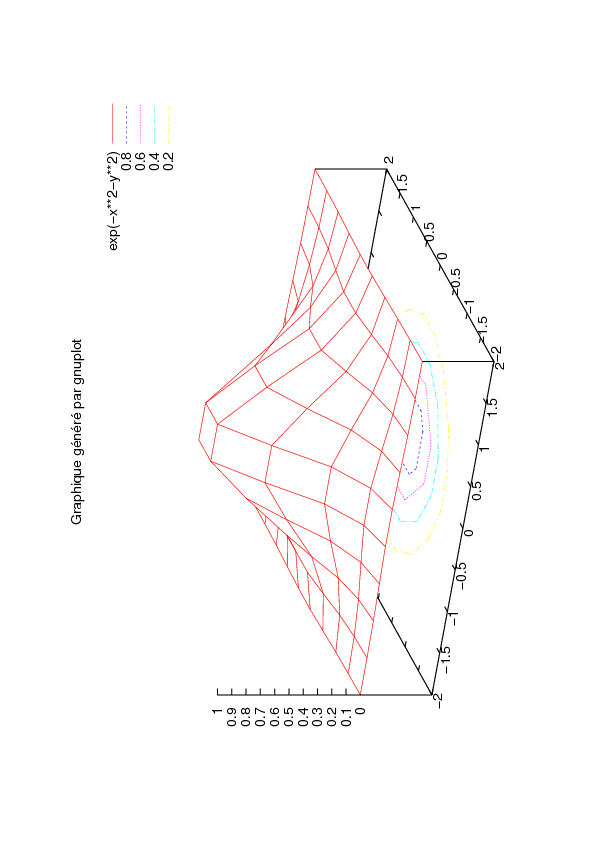
\includegraphics[width=.5\textwidth, angle=-90]{material/graphe}
  \caption{Un exemple de graphique flottant}
  \label{float}
\end{figure}


\section{Et celui d'un graphique non-flottant}

\begin{center}
  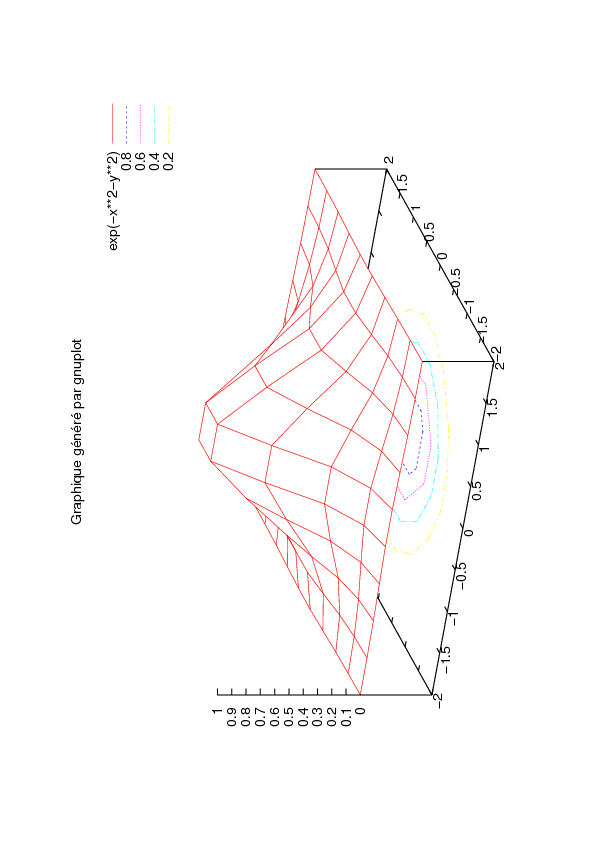
\includegraphics[width=.5\textwidth, angle=-90]{material/graphe}
  \label{nofloat}
\end{center}

Le seul moyen pour attribuer un titre à un graphique est de le faire
flotter (c'est voulu). La commande \verb1\caption1 ne peut pas être
utilisée en dehors de l'environnement \verb1figure1. Il est de toutes
façons recommandé de \emph{toujours} faire flotter les graphiques.


\section{Faire référence à un graphique}

\begin{itemize}
\item Ne fonctionne que pour les graphiques flottants (i.e. ceux à qui on
  attribue un numéro, par exemple, le graphique \ref{float}). S'ils ne flottent
  pas (par exemple le second graphique dans notre exemple), c'est le numéro de
  section (cf.  section \ref{nofloat}) qui sera utilisé par l'appel
  \verb1\ref{...}1. On peut bien sûr utiliser également le numéro de page (cf.
  page \pageref{nofloat}).
\item \verb1\label{nom}1 : attribue un label au graphique.
  \begin{itemize}
  \item En général, on fait précéder les labels des graphiques de
    \emph{\selectlanguage{english}fig:} (pour \emph{figure}, mais c'est juste
    une convention d'usage), par exemple \verb1\label{fig:data}1.
  \end{itemize}
\item \verb1\ref{nom}1 : effectue un renvoi vers le numéro du graphique qui
  correspond au repère \emph{nom}.
\item Pour les graphiques flottants (Attention, s'ils ne flottent pas,
  ils ne disposent pas d'un numéro ; on peut cepedendant renvoyer à la
  page sur laquelle ils apparaissent), il convient de situer l'appel
  \verb1\label{nom}1 à l'intérieur de l'environnement \emph{figure},
  juste après la commande \verb1\caption{}1.

  \begin{exemple}[H]
    \caption{Référence à un graphique}
    \label{ex:reftab}
\begin{verbatim}
\begin{figure}
  \includegraphics[width=.5\textwidth, angle=-90]{fichier}
  \caption{Titre attribué au graphique.}
  \label{fig:data}.
\end{figure}
\end{verbatim}
  \end{exemple}
  
\item \verb1\pageref{nom}1 : effectue un renvoi vers le numéro de la page qui
  correspond au repère \emph{nom}. Pour le reste, il fonctionne exactement de la
  même manière que \verb1\ref1.
\end{itemize}


Par exemple, le renvoi à ce graphique se traduirait par :

\begin{exemple}[H]
  \caption{Référence à un graphique}
  \label{ex:reftab}
\begin{verbatim}
On voit dans la Figure~/ref{fig:data}, p.\pageref{fig:data}...
\end{verbatim}
\end{exemple}


Notez l'usage du caractère \og \verb1~1 \fg (tilde) qui permet
d'insérer un espace insécable (pour obtenir ce caractère, on utilise
AltGr+2 sur un PC et Command+SHIFT+N sur un Mac).



\chapter{Les objets flottants : insertion de tableaux}
\label{cha:tableaux}
\begin{center}
  \begin{minipage}[r]{0.5\linewidth}
    Les tableaux sont aussi des objets qui peuvent flotter. Nous
    allons donc retrouver certains points abordés dans le cas des
    graphiques. Mais vous allez aussi apprendre à créer des tableaux
    de données. Cette partie devrait vous prendre beaucoup de temps
    car, si les tableaux produits par LaTeX peuvent être d'une qualité
    typographique exceptionnelle, ceci demandera beaucoup de travail
    de votre part.
  \end{minipage}
\end{center}



\section{Les tableaux}
\label{tableaux}

\vfill 

Comme pour les graphiques, deux points indépendants sont à considérer :

\begin{itemize}
\item La création d'un tableau dans un document \LaTeX\ (cf.~\ref{tabular}).
\item Le positionnement du tableau et de son titre dans le document (retour à la
  notion de flottant, cf.~\ref{table}).
\end{itemize}

\vfill







\section{Créer un tableau avec les outils standards}
\label{tabular}

\vfill

\begin{boxedminipage}{\textwidth}
\begin{verbatim}
\begin{tabular}{spécification des colonnes}
donnée & donnée & donnée & ... & donnée \\
donnée & donnée & donnée & ... & donnée \\
...
\end{tabular}
\end{verbatim}
\end{boxedminipage}

\begin{itemize}
\item Instructions utiles
  \begin{itemize}
  \item \verb1\hline1 : trace une ligne horizontale sur toute la largeur du
    tableau;
  \item \verb1\cline{N-M}1 : trace une ligne horizontale des colonnes N à M;
  \item \verb1\multicolumn{nbcols}{format}{Texte étendu sur plusieurs colonnes}1
  \item la déclaration des colonnes se fait avec les lettres \emph{c,
      l, r} (center, left, right). On indique autant de lettres que
    l'on veut de colonnes, chaque lettre indique l'alignement du texte
    dans la colonne;
  \item Les \verb1&1 servent à sépararer les colonnes;
  \item On indique la fin de ligne par \verb1\\1.
  \end{itemize}
\end{itemize}

%%Nous allons voir quelques exemples de l'utilisation de \emph{tabular} :
\vfill

\section{Exercices}

\begin{itemize}
\item Construisez, sur papier, un tableau très simple (3 colonnes, 5
  lignes) et reproduisez le avec \LaTeX\ en traçant toutes les lignes
  verticales et horizontales;
\item Reproduisez ce même tableau en supprimant toutes les lignes;
\item Reproduisez pour finir ce même tableau en n'introduisant que les
  lignes horizontales;
\item Reproduisez ensuite le tableau présenté ci-dessous en utilisant
  les instructions nécessaires.
\end{itemize}

\begin{center}
  \begin{tabular}{|l|cr|l|} \hline
    Alignement à gauche & Données centrées & et à droite & Largeur imposée\\ \cline{2-3}
    Donnée & \multicolumn{2}{|c|}{Donnée} & \\ \hline
    1.10 & 2.20 & 3.20 & 4.69 \\
    1.10 & 2.20 & 3.20 & 4.69 \\
    1.10 & 2.20 & 3.20 & 4.69 \\ \hline
  \end{tabular}
\end{center}


\section{L'environnement \emph{tabular}: réponse à la question
  précédente}

\begin{boxedminipage}{\textwidth}
\footnotesize
\begin{verbatim}
\begin{center}
  \begin{tabular}{|l|cr|l|} \hline
    Alignement à gauche & Données centrées & et à droite & Largeur imposée\\ \cline{2-3}
    Donnée & \multicolumn{2}{|c|}{Donnée} & \\ \hline
    1.10 & 2.20 & 3.20 & 4.69 \\
    1.10 & 2.20 & 3.20 & 4.69 \\
    1.10 & 2.20 & 3.20 & 4.69 \\ \hline
  \end{tabular}
\end{center}
\end{verbatim}
\end{boxedminipage}

\begin{center}
  \begin{tabular}{|l|cr|l|} \hline
    Alignement à gauche & Données centrées & et à droite & Largeur imposée\\ \cline{2-3}
    Donnée & \multicolumn{2}{|c|}{Donnée} & \\ \hline
    1.10 & 2.20 & 3.20 & 4.69 \\
    1.10 & 2.20 & 3.20 & 4.69 \\
    1.10 & 2.20 & 3.20 & 4.69 \\ \hline
  \end{tabular}
\end{center}

%% Problèmes de tabular :

%% - contrôle de la largeur des cellules (array, tabularx)
%% - centrage vertical du texte dans la cellule (array)
%% - écartement entre le texte et les lignes horizontales (booktabs)

%% - tableaux longs à introduire sur plusieurs pages (longtable)

%% - multirow : regroupement vertical de cellules (doit-on vraiment l'aborder ?)


\section{Quelques problèmes centraux dans la composition d'un tableau}

\vfill

\subsection{Largeur des cellules}

Pour les colonnes contenant du texte de longueur importante, il faut
indiquer la largeur de colonne souhaitée, sinon l'on obtient quelque
chose d'assez désagréable : \LaTeX\ attribue à la cellule la largeur
du texte qu'elle contient (ce qui peut être vraiment grand !).

\subsection{Alignement vertical du texte}

L'environnement \emph{tabular} standard ne permet pas de contrôler
l'alignement vertical. Le texte est nécessairement aligné avec le haut
de la cellule.

\subsection{\'Ecartement texte / ligne horizontale}

Certaines lettres (les majuscules) touchent la ligne horizontale qui les domine.

\vfill


\section{Illustrations}

\subsection{Largeur des cellules}

\begin{boxedminipage}{\textwidth}
\begin{verbatim}
\begin{tabular}{|l|cr|c|} \hline
  Donnée & Donnée & Donnée & Ici un texte relativement long...\\ \hline
\end{tabular}
\end{verbatim}
\end{boxedminipage}

\begin{center}
  \begin{tabular}{|l|cr|c|} \hline
    Donnée & Donnée & Donnée & Sinon, \LaTeX\ adapte la taille de la colonne à la taille du texte. Ce qui peut poser des problèmes.\\ \hline
    % Donnée & Donnée & Donnée & \\ \hline
  \end{tabular}
\end{center}

\subsection{Alignement vertical}

\begin{tabular}{|p{.5\textwidth}|ccc|} \hline
  Texte relativement long blah blah blah blah blah blah blah blah blah blah blah blah blah blah blah blah blah blah & A & A & A \tabularnewline \cline{2-4}
  & A & A & A \tabularnewline \cline{2-4}
  & B & B & B \tabularnewline \hline
\end{tabular}


\subsection{Espacement caractère / ligne}

Le problème de l'espacement entre les caractères et la ligne
horizontale est manifeste dans ces deux exemples.



\section{Contrôle de la largeur des colonnes}

\vfill

On dispose de plusieurs solutions dont le choix dépend de la
situation et des préférences de l'utilisateur.


\begin{enumerate}
\item L'utilisateur souhaite laisser \LaTeX\ gérer lui-même la largeur des
  colonnes (gestion automatique) : utiliser l'extension \emph{tabularx}
\item L'utilisateur souhaite avoir le contrôle total de la largeur de chaque
  colonne : utiliser l'extension \emph{array}.
\end{enumerate}

Deux possibilités peuvent apparaître :
\begin{enumerate}
\item \label{toutes}Toutes les cases de la colonne vont contenir un texte de
  ce type. On utilise une technique de définition des colonnes avec l'appel à
  l'extension \emph{array}.
\item \label{titre}Seule une case (souvent dans la ligne de titre ou
  dans la colonne de gauche) contient un texte long, le reste
  contenant des données (par exemple numériques). On pourra utiliser
  soit \emph{array}, soit \emph{tabularx}.
\end{enumerate}

Pour le problème de l'espacement entre lignes horizontales et
caractères, on utilisera l'extension \emph{booktab}.

\vfill




% \section{Première situation}

% \begin{boxedminipage}{\textwidth}
% \begin{verbatim}
% \begin{center}
%   \begin{tabular}{|l|cr|p{.3\textwidth}|} \hline
%     Donnée & Donnée & Donnée & \begin{center}Et une case...\end{center}\\ \hline
%     ...
%     Donnée & \multicolumn{2}{|c|}{Donnée} & \\ \hline
%   \end{tabular}
% \end{center}
% \end{verbatim}
% \end{boxedminipage}


% \begin{center}
%   \begin{tabular}{|l|cr|p{.3\textwidth}|} \hline
%     Donnée & Donnée & Donnée & \begin{center}Et une case du tableau qui contient beaucoup de texte. La dimension de cette case est fixée, pas automatique.\end{center}\\ \hline
%     Donnée & Donnée & Donnée & \begin{center}Et une case du tableau qui contient beaucoup de texte. La dimension de cette case est fixée, pas automatique.\end{center}\\ \hline
%     Donnée & \multicolumn{2}{|c|}{Donnée} & \\ \hline
%   \end{tabular}
% \end{center}







% \section{Seconde situation}

%  \begin{boxedminipage}{\textwidth}
%  \begin{verbatim}
%  \begin{center}
%  \begin{tabular}{|l|cr|r|} \hline
%  Don. & Don. & Don. & \begin{minipage}{.4\textwidth} TEXTE \end{minipage}\\ \hline
%  1.10 & 2.20 & 3.20 & 4.69 \\
%  1.10 & 2.20 & 3.20 & 4.69 \\
%  1.10 & 2.20 & 3.20 & 4.69 \\ \hline
%  \end{tabular}
%  \end{center}
%  \end{verbatim}
%  \end{boxedminipage}

%  \begin{center}
%  \begin{tabular}{|l|cr|r|} \hline
%  Donnée & Donnée & Donnée & \begin{minipage}{.4\textwidth}Et une case du tableau qui contient beaucoup de texte. La dimension de cette case est fixée, pas automatique.\end{minipage}\\ \hline
%  1.10 & 2.20 & 3.20 & 4.69 \\
%  1.10 & 2.20 & 3.20 & 4.69 \\
%  1.10 & 2.20 & 3.20 & 4.69 \\ \hline
%  \end{tabular}
%  \end{center}

%  Quelques problèmes persistent :

%  \begin{itemize}
%  \item Comment joindre deux cellules verticalement ? (multirow)
%  \item Comment centrer le texte verticalement dans les cases ? (array)
%    \begin{itemize}
%    \item Remarquez qu'en utilisant minipage au lieu de \verb1p{largeur}1, les
%      autres cellules sont centrées verticalement.
%    \end{itemize}
%  \item Le texte des données chevauche les lignes horizontales du tableau
%    (booktab)
%  \end{itemize}







\section{L'extension \emph{tabularx}}

\vfill

\begin{itemize}
  
\item On appelle l'extension \emph{tabularx} et on utilise
  l'environnement \emph{tabularx}.

\begin{boxedminipage}{\textwidth}
\begin{verbatim}
\usepackage{tabularx}
...
\begin{tabularx}{.9\textwidth}{Xccc}
...
\end{tabularx}
\end{verbatim}
\end{boxedminipage}


\item On indique la largeur souhaitée pour tout le tableau (par
  exemple 90\% de la largeur de la page) et on marque les colonnes à
  faire varier automatiquement par un X. Les autres colonnes prennent
  la largeur du texte qu'elles contiennent (fonctionnement classique
  de \LaTeX).

\begin{tabularx}{.9\textwidth}{|X|ccc|} \hline
Texte relativement long blah blah blah blah blah blah blah blah blah blah blah blah blah blah blah blah blah blah & A & A & A \tabularnewline \cline{2-4}
& A & A & A \tabularnewline \cline{2-4}
& B & B & B \tabularnewline \hline
\end{tabularx}

\item Problèmes de tabularx : ne permet pas de contrôler l'alignement
  vertical du texte dans les cellules (toujours aligné en
  haut). L'apparence finale est --de mon point de vue-- nettement
  moins agréable qu'avec le contrôle fourni par \emph{array}.

\end{itemize}

\vfill




\section{L'extension \emph{array}}

\begin{itemize}
\item On appelle l'extension \emph{array} dans l'en-tête du document par
  \verb1\usepackage{array}1.
\item L'utilisation est ensuite exactement la même que dans la version standard
  de \LaTeX. (environnement tabular).
\item Par exemple :

  \begin{boxedminipage}{\textwidth}
\small
\begin{verbatim}
\begin{tabular}{b{.5\textwidth}b{.1\textwidth}cc} \hline
Texte relativement long blah ... & A & A & A \\ \cline{2-4}
                            & A & A & A \\ \cline{2-4}
                            & B & B & B \\ \hline
\end{tabular}
\end{verbatim}
  \end{boxedminipage}

\item donne :

\begin{tabular}{b{.5\textwidth}b{.1\textwidth}cc} \hline
Texte relativement long blah blah blah blah blah blah blah blah blah blah blah blah blah blah blah blah blah blah & A & A & A \tabularnewline \cline{2-4}
& A & A & A \\ \cline{2-4}
& B & B & B \\ \hline
\end{tabular}

\item Chaque colonne se voit attribuer une largeur fixée par le
  rédacteur. Le texte qui est plus large que cette colonne est
  \emph{plié} aux dimensions de la colonne. Vous remarquez que les
  déclarations des colonnes sont, pour certaines, très différentes :
  on a remplacé une lettre (c, l ou r) par la commande
  \verb1b{.5\textwidth}1 par exemple pour la première colonne. Les
  colonnes déclarées c, l ou r continuent d'être gérées classiquement
  (largeur automatique attribuée par \LaTeX).

\end{itemize}

\section{Améliorer l'usage de l'extension \emph{array}}

\begin{itemize}
\item \emph{array} fournit la possibilité de définir \emph{au préalable} des
  déclarations pour les colonnes.
\item L'instruction \verb1\newcolumntype{lettre}{définition}1 permet, avant la
  composition du tableau, de définir les caractéristiques des colonnes en leur
  attribuant des types.
\item Exemple :
\begin{verbatim}
\newcolumntype{t}{b{.40\textwidth}}
\newcolumntype{d}{b{.10\textwidth}}
\end{verbatim}
\item Définit 2 nouveaux types de colonnes : t (40\% de la largeur du
  texte, texte aligné sur le bas de la cellule) et d (10\% de la
  largeur du texte et texte également aligné sur le bas de la
  cellule).
\item On peut alors utiliser les lettres \emph{t} et \emph{d} à la place (ou en
  alternance) des lettres \emph{l}, \emph{c} ou \emph{r}.
\item Cette fonctionnalité permet même de modifier d'autres caractéristiques des
  cellules : notamment la police utilisée, la taille\ldots
\begin{verbatim}
\newcolumntype{t}{>{\slshape}b{.40\textwidth}}
\newcolumntype{d}{>{\centering\ttfamily\small}b{.10\textwidth}}
\end{verbatim}
\item Attention cependant : remplacer \verb1\\1 par \verb1\tabularnewline1 pour
  marquer les fins de lignes du tableau.
\end{itemize}




\section{Règle d'utilisation de \emph{newcolumntype}}

\begin{center}
\begin{verbatim}
    \newcolumntype{t}{>{formatage}b{.40\textwidth}}
\end{verbatim}
\end{center}

\begin{itemize}
\item Où le formatage peut servir à déclarer un choix de type de police :
  \begin{itemize}
  \item \verb1\rmfamily1 : Roman (= Serif, cf. Times)
  \item \verb1\sffamily1 : Sans Serif (cf. Helvetica)
  \item \verb1\ttfamily1 : Typewriter (cf. Courier) \emph{Particulièrement utile
      pour les colonnes de chiffres}
  \end{itemize}
\item une orientation des caractères :
  \begin{itemize}
  \item \verb1\slshape1 : Slanted (italique)
  \item \verb1\upshape1 : Droit (par défaut)
  \item \verb1\scshape1 : Small Caps (petites capitales)
  \end{itemize}
\item une graisse :
  \begin{itemize}
  \item \verb1\bfseries1 : Gras
  \end{itemize}
\item un alignement horizontal :
  \begin{itemize}
  \item \verb1\centering1 : Centré
  \item \verb1\raggedleft1 : Repoussé depuis la gauche (Aligné à droite)
  \item \verb1\raggedright1 : Repoussé depuis la droite (Aligné à gauche)
  \end{itemize}
\item une taille de caractères :
  \begin{itemize}
  \item \verb1\tiny1 : du plus petit
  \item \verb1\scriptsize1 : \ldots
  \item \verb1\footnotesize1 : \ldots
  \item \verb1\small1 : \ldots
  \item \verb1\normalsize1 : \ldots
  \item \verb1\large1 : \ldots
  \item \verb1\Large1 : \ldots
  \item \verb1\LARGE1 : \ldots
  \item \verb1\huge1 : \ldots
  \item \verb1\Huge1 : au plus grand
  \end{itemize}
\end{itemize}

Exemple : \verb2\newcolumntype{d}{>{\ttfamily\raggedleft}b{.1\textwidth}}2

Ces déclarations sont des commandes standard de \LaTeX\ (on peut les
utiliser ailleurs pour changer les caractéristiques d'un texte par
exemple).

\section{Un exemple plus complet : alignement sur le bas de la cellule}

\begin{boxedminipage}{\textwidth}
\begin{verbatim}
\newcolumntype{t}{>{\slshape\centering}b{.40\textwidth}}
\newcolumntype{d}{>{\ttfamily\raggedleft}p{.10\textwidth}}

\begin{center}
\begin{tabular}{tddd} \hline
Texte relativement long blah... & A & A & A \tabularnewline \cline{2-4}
        & A & A & A \tabularnewline \cline{2-4}
        & B & B & B \tabularnewline \hline
\end{tabular}
\end{center}
\end{verbatim}
\end{boxedminipage}

\newcolumntype{t}{>{\slshape\centering}b{.40\textwidth}}
\newcolumntype{d}{>{\ttfamily\raggedleft}p{.10\textwidth}}

\begin{center}
\begin{tabular}{tddd} \hline
Texte relativement long blah blah blah blah blah blah blah blah blah blah blah blah blah blah blah blah blah blah & A & A & A \tabularnewline \cline{2-4}
& A & A & A \tabularnewline \cline{2-4}
& B & B & B \tabularnewline \hline
\end{tabular}
\end{center}



\section{Un exemple plus complet : alignement sur le milieu vertical
  de la cellule}

\begin{boxedminipage}{\textwidth}
\begin{verbatim}
\newcolumntype{t}{>{\slshape\centering}m{.40\textwidth}}
\newcolumntype{d}{>{\ttfamily\raggedleft}p{.10\textwidth}}

\begin{center}
\begin{tabular}{tddd} \hline
Texte relativement long blah... & A & A & A \tabularnewline \cline{2-4}
        & A & A & A \tabularnewline \cline{2-4}
        & B & B & B \tabularnewline \hline
\end{tabular}
\end{center}
\end{verbatim}
\end{boxedminipage}

\newcolumntype{t}{>{\slshape\centering}m{.40\textwidth}}
\newcolumntype{d}{>{\ttfamily\raggedleft}p{.10\textwidth}}

\begin{center}
\begin{tabular}{tddd} \hline
Texte relativement long blah blah blah blah blah blah blah blah blah blah blah blah blah blah blah blah blah blah & A & A & A \tabularnewline \cline{2-4}
& A & A & A \tabularnewline \cline{2-4}
& B & B & B \tabularnewline \hline
\end{tabular}
\end{center}







\section{Notes sur l'utilisation de l'extension \emph{array}}

\vfill{}

\begin{itemize}
\item Attention : la largeur de la colonne est en réalité la largeur du texte
  contenu dans la colonne (non compris les espaces gauche et droit autour du
  texte). On risque donc de dépasser la largeur du texte si la somme des
  largeurs de colonnes est égale à 100\% (il suffit de le savoir).
\item L'usage de l'instruction \verb2b{.1\textwidth}2 indique que la colonne
  doit avoir une largeur équivalente à 10\% de la largeur totale du texte sur la
  page \emph{et} que ce texte doit être aligné sur la bas de la cellule (b =
  bottom). On peut aussi centrer le texte verticalement (remplacer \emph{b} par
  \emph{m}).  \emph{p} produit le fonctionnement standard (alignement sur le
  haut de la cellule).
\item La déclaration du type d'alignement vertical est attribuée à une
  colonne mais, évidemment, son effet va porter sur les lignes ! Il
  faut le comprendre comme une indication du type d'alignement qu'on
  va obtenir du texte contenu dans les autres colonnes par rapport à
  la cellule correspondante : si une cellule de la colonne 1 (type
  \verb1t1) contient beaucoup de texte, les autres cellules de la même
  ligne seront alignées sur le bas de cette première cellule. Dans les
  exemples précédents, si une cellule des 3 colonnes de gauche
  contenait beaucoup de texte, le texte des autres cellules serait
  aligné sur le haut de cette cellule !
 \item Noter qu'il est tout à fait possible d'alterner, dans un même document,
   l'usage des environnements \emph{tabular} et \emph{tabularx} en fonction des
   besoins.
\end{itemize}

\vfill{}



%% \section{L'extension \emph{multirow}}

%% \vfill

%% Utilisation de l'extension :

%% \begin{boxedminipage}{\textwidth}
%% \begin{verbatim}
%% \usepackage{multirow}

%% \begin{tabular}{lr} \hline
%% \multirow{nbrows}{largeur}[décalage]{Texte} & donnée \\
%%                                     & donnée \\ \hline
%% \end{tabular}
%% \end{verbatim}
%% \end{boxedminipage}

%% Nous verrons quel peut être l'usage de l'option [décalage] tout à l'heure. Pour
%% l'instant, nous souhaitons essentiellement voir comment écrire du texte dans
%% deux cellules (comment regrouper des cellules).

%% \vfill

%% \section{Utilisation de \emph{multirow}}


%% \begin{boxedminipage}{\textwidth}
%% \begin{verbatim}
%% \begin{center}
%% \begin{tabular}{|c|cp{.3\textwidth}|} \hline
%% \multirow{2}{*}{Titre commun} & Donnée & Un texte relativement ... \\ \cline{2-3}
%%                         & Donnée & Donnée \\ \hline
%% \multirow{2}{.2\textwidth}{Titre long} & Donnée & Un texte ... \\ \cline{2-3}
%%                         & Donnée & Donnée \\ \hline
%% \end{tabular}
%% \end{center}
%% \end{verbatim}
%% \end{boxedminipage}



%% \begin{center}
%% \begin{tabular}{|c|cp{.3\textwidth}|} \hline
%% \multirow{2}{*}{Titre commun} & Donnée & Un texte relativement long pour voir l'effet des cellules qui contiennent beaucoup de texte sur la mise en page du tableau. \\ \cline{2-3}
%%                         & Donnée & Donnée \\ \hline
%% \multirow{2}{.2\textwidth}{Titre commun qui contient plus de texte que n'en pourrait contenir une seule cellule, vraiment beacoup plus} & Donnée & Un texte relativement long pour voir l'effet des cellules qui contiennent beaucoup de texte sur la mise en page du tableau. \\ \cline{2-3}
%%                         & Donnée & Donnée \\ \hline
%% \end{tabular}
%% \end{center}

%% %% \begin{center}
%% %% \begin{tabular}{|c|cc|} \hline
%% %% \multirow{2}{*}{Titre commun} & Donnée & \begin{minipage}{.3\textwidth}Un texte relativement long pour voir l'effet des cellules qui contiennent beaucoup de texte sur la mise en page du tableau.\end{minipage} \\ \cline{2-3}
%% %%                         & Donnée & Donnée \\ \hline
%% %% \multirow{2}{.2\textwidth}{Titre commun qui contient plus de texte que n'en pourrait contenir une seule cellule} & Donnée & \begin{minipage}{.3\textwidth}Un texte relativement long pour voir l'effet des cellules qui contiennent beaucoup de texte sur la mise en page du tableau.\end{minipage} \\ \cline{2-3}
%% %%                         & Donnée & Donnée \\ \hline
%% %% \end{tabular}
%% %% \end{center}


%% Elle permet d'améliorer la mise en page du tableau, notamment lorsque celui-ci
%% contient des cellules qui doivent inclure une grande quantité de texte. Elle
%% utilise la même syntaxe que \emph{tabular}.

%% On l'appelle dans l'en-tête du document par \verb1\usepackage{array}1 et on
%% définit la largeur des cellules pour lesquelles on ne souhaite pas de contrôle
%% automatique en utilisant \verb1m{largeur}1 au lieu de \verb1p{largeur}1.

%% Pour faire intervenir \emph{array}, on définit la largeur d'au-moins une
%% cellule.


%% Avec \emph{array} (\verb1\begin{tabular}{|l|cr|m{.3\textwidth}|} \hline1) :
  
%%   \begin{boxedminipage}{\textwidth}
%% \begin{verbatim}
%% \begin{tabular}{|l|cr|m{.3\textwidth}|} \hline
%% Donnée & Donnée & Donnée & \begin{center}Et une case...\end{center}\\ \cline{2-3}
%% Donnée & Donnée & Donnée & \\ \hline
%% \end{tabular}
%% \end{verbatim}
%%   \end{boxedminipage}

%% \begin{center}
%% \begin{tabular}{|l|cr|m{.3\textwidth}|} \hline
%% Donnée & Donnée & Donnée & \begin{center}Et une case du tableau qui contient beaucoup de texte. La dimension de cette case est fixée, pas automatique.\end{center}\\ \cline{2-3}
%% Donnée & Donnée & Donnée & \\ \hline
%% \end{tabular}
%% \end{center}

%% \newpage

%% et sans \emph{array} (\verb1\begin{tabular}{|l|cr|p{.3\textwidth}|} \hline1) :

%%   \begin{boxedminipage}{\textwidth}
%% \begin{verbatim}
%% \begin{tabular}{|l|cr|p{.3\textwidth}|} \hline
%% Donnée & Donnée & Donnée & \begin{center}Et une case...\end{center}\\ \cline{2-3}
%% Donnée & Donnée & Donnée & \\ \hline
%% \end{tabular}
%% \end{verbatim}
%%   \end{boxedminipage}

%% \begin{center}
%% \begin{tabular}{|l|cr|p{.3\textwidth}|} \hline
%% Donnée & Donnée & Donnée & \begin{center}Et une case du tableau qui contient beaucoup de texte. La dimension de cette case est fixée, pas automatique.\end{center}\\ \cline{2-3}
%% Donnée & Donnée & Donnée & \\ \hline
%% \end{tabular}
%% \end{center}


\section{Le problème du chevauchement lettres / lignes}

Vous avez probablement remarqué que les lignes horizontales des tableaux
chevauchent le haut de certaines lettres.


\begin{itemize}
\item Pour empêcher les lettres de chevaucher les lignes horizontales du
  tableau, on peut introduire une instruction (à n'importe quel endroit du
  document mais en général dans l'en-tête):
  \begin{itemize}
  \item \verb1\setlength{\extrarowheight}{dimension}1
  \end{itemize}
\item Dans le tableau précédent, les lettres hautes (notamment les majuscules)
  touchent les lignes horizontales qui les dominent.
\item Si on ajoute \verb1\setlength{\extrarowheight}{0.3em}1, dans l'en-tête du
  document ou avant de composer le tableau, on obtient :
  \setlength{\extrarowheight}{0.3em}

\begin{center}
\begin{tabular}{|t|ddd|} \hline
Texte relativement long blah blah blah blah blah blah blah blah blah blah blah blah blah blah blah blah blah blah & A & A & A \tabularnewline \cline{2-4}
& A & A & A \tabularnewline \cline{2-4}
& B & B & B \tabularnewline \hline
\end{tabular}
\end{center}

% \item Mais cette procédure peut (lorsqu'on utilise des lignes
%   verticales, mais cf p.\ref{regles-table}) produire des vides.
\end{itemize}

Mais l'outil le plus intéressant pour construire les tableaux (en
combinaison avec \emph{array}) est l'extension \emph{booktabs},
développée pour construire des tableaux de qualité pour la publication
de documents écrits.


\section{L'extension \emph{booktabs}}
\label{booktab}
\setlength{\extrarowheight}{0ex}

\vfill
\begin{itemize}
\item \verb1\usepackage{booktabs}1
\item L'extension \emph{booktabs} s'occupe de formater un tableau en respectant
  scrupuleusement les nécessités typographiques en vigueur dans l'édition.
  \begin{itemize}
  \item Amélioration de la gestion des espaces entre les lignes (pas besoin de
    modifier arbitrairement l'espacement entre les lignes et le texte).
  \item Possibilité de faire varier l'épaisseur des lignes (épaisse en haut et
    en bas, fine à l'intérieur du tableau).
  \item Compatible avec \emph{array} (on peut fixer la largeur des colonnes et
    leur alignement vertical par exemple).
  \item Fonctionne aussi avec \emph{longtable} (cf. p.\ref{longtable}).
%  \item Permet d'insérer des sauts de lignes dans un texte relativement long.
  \end{itemize}
\item Notez qu'un tableau de données NE DOIT PAS comporter de lignes
  verticales.
\end{itemize}
\vfill
\newpage

\section{Différences entre \emph{array} et \emph{booktabs}}

\begin{itemize}
\item \emph{array} et \emph{booktabs} peuvent être utilisés simultanément.
\item Mais \emph{booktabs} doit être considéré comme une couche supplémentaire
  qui améliore la mise en page.
  
  \begin{center}
    \begin{tabular}{l!{$\rightarrow$}l} \toprule
      \emph{array} & \emph{booktabs} \tabularnewline \midrule
      \verb1\hline1 & \verb1\toprule1 \tabularnewline
      & \verb1\midrule1 \tabularnewline
      & \verb1\bottomrule1 \tabularnewline \midrule
      \verb1\cline{N-M}1 & \verb1\cmidrule{N-M}1 \tabularnewline \bottomrule
    \end{tabular}
  \end{center}
\end{itemize}

Notez que les épaisseurs de lignes peuvent ne pas apparaître
correctement à l'écran (visualisation PDF) mais apparaîtront
correctement à l'impression.


\section{Exemple d'utilisation de \emph{booktabs}}

\begin{boxedminipage}{\textwidth}
\begin{verbatim}
\usepackage{booktabs}

\begin{tabular}{lcrrr} \toprule
  & & Condition 1 & Condition 2 & Condition 3 \tabularnewline \midrule
  Expérience 1 & Temps de réaction (en ms) & 600 & 700 & 800 \tabularnewline
  & Taux d'erreur (en \%)  & 14 & 10 & 4 \tabularnewline \cmidrule{2-5}
  Expérience 2 & Temps de réaction (en ms) & 700 & 700 & 700 \tabularnewline
  & Taux d'erreur (en \%)  & 14 & 24 & 34 \tabularnewline \midrule
\end{tabular}
\end{verbatim}
\end{boxedminipage}

\begin{center}
  \begin{tabular}{lcrrr} \toprule
    & & Condition 1 & Condition 2 & Condition 3 \tabularnewline \midrule
    Expérience 1 & Temps de réaction (en ms) & 600 & 700 & 800 \tabularnewline
    & Taux d'erreur (en \%)  & 14 & 10 & 4 \tabularnewline \cmidrule{2-5}
    Expérience 2 & Temps de réaction (en ms) & 700 & 700 & 700 \tabularnewline
    & Taux d'erreur (en \%)  & 14 & 24 & 34 \tabularnewline \midrule
%%     Et même si l'on a \emph{vraiment} besoin d'insérer un texte relativement long dans cette cellule, son formatage est correct & Temps de réaction (en ms) & 700 & 700 & 700 \tabularnewline
%%     & Taux d'erreur (en \%)  & 14 & 24 & 34 \tabularnewline \bottomrule
%%     \multicolumn{3}{l}{\begin{minipage}{.6\textwidth}D'ailleurs un formatage avec extension de la cellule sur la ligne serait certainement plus agréable à lire. Même si le texte qu'elle contient est extrêmement long.\end{minipage}} & &  \\
%%     & Temps de réaction (en ms) & 700 & 700 & 700 \\
%%     & Taux d'erreur (en \%)  & 14 & 24 & 34 \\ \bottomrule
  \end{tabular}
\end{center}


\section{Et en collaboration avec \emph{array}\ldots}

\newcolumntype{t}{>{\slshape\raggedright}b{.20\textwidth}}
\newcolumntype{s}{>{\sffamily}c}
\newcolumntype{d}{>{\ttfamily}r}

\begin{boxedminipage}{\textwidth}
\begin{verbatim}
\newcolumntype{t}{>{\slshape\raggedright}b{.20\textwidth}}
\newcolumntype{s}{>{\sffamily}c}
\newcolumntype{d}{>{\ttfamily}r}

\begin{tabular}{lcrrr} \toprule
  & & Condition 1 & Condition 2 & Condition 3 \tabularnewline \midrule
  Expérience 1 & Temps de réaction (en ms) & 600 & 700 & 800 \tabularnewline
  & Taux d'erreur (en \%)  & 14 & 10 & 4 \tabularnewline \cmidrule{2-5}
  Expérience 2 & Temps de réaction (en ms) & 700 & 700 & 700 \tabularnewline
  & Taux d'erreur (en \%)  & 14 & 24 & 34 \tabularnewline \midrule
\end{tabular}
\end{verbatim}
\end{boxedminipage}

\begin{center}
  \begin{tabular}{tsddd} \toprule
    & & Condition 1 & Condition 2 & Condition 3 \tabularnewline \midrule
    Expérience 1 & Temps de réaction (en ms) & 600 & 700 & 800 \tabularnewline
    & Taux d'erreur (en \%)  & 14 & 10 & 4 \tabularnewline \cmidrule{2-5}
    Expérience 2 & Temps de réaction (en ms) & 700 & 700 & 700 \tabularnewline
    & Taux d'erreur (en \%)  & 14 & 24 & 34 \tabularnewline \midrule
%%     Et même si l'on a \emph{vraiment} besoin d'insérer un texte relativement long dans cette cellule, son formatage est correct & Temps de réaction (en ms) & 700 & 700 & 700 \tabularnewline
%%     & Taux d'erreur (en \%)  & 14 & 24 & 34 \tabularnewline \bottomrule
%%     \multicolumn{3}{l}{\begin{minipage}{.6\textwidth}D'ailleurs un formatage avec extension de la cellule sur la ligne serait certainement plus agréable à lire. Même si le texte qu'elle contient est extrêmement long.\end{minipage}} & &  \\
%%     & Temps de réaction (en ms) & 700 & 700 & 700 \\
%%     & Taux d'erreur (en \%)  & 14 & 24 & 34 \\ \bottomrule
  \end{tabular}
\end{center}


% \section{\ldots et avec \emph{tabularx}}

% \begin{boxedminipage}{\textwidth}
% \begin{verbatim}
% \newcolumntype{s}{>{\slshape\centering}m{.2\textwidth}}

% \begin{tabular}{Xsrrr} \toprule
%   & & Condition 1 & Condition 2 & Condition 3 \tabularnewline \midrule
%   Expérience 1 & Temps de réaction (en ms) & 600 & 700 & 800 \tabularnewline
%   & Taux d'erreur (en \%)  & 14 & 10 & 4 \tabularnewline \cmidrule{2-5}
%   Expérience 2 & Temps de réaction (en ms) & 700 & 700 & 700 \tabularnewline
%   & Taux d'erreur (en \%)  & 14 & 24 & 34 \tabularnewline \midrule
% \end{tabular}
% \end{verbatim}
% \end{boxedminipage}

% %\newcolumntype{s}{>{\slshape}c}
% \newcolumntype{s}{>{\slshape\centering}m{.3\textwidth}}
% \begin{center}
%   \begin{tabularx}{.9\textwidth}{Xsrrr} \toprule
%     & & Condition 1 & Condition 2 & Condition 3 \\ \midrule
%     Expérience 1 & Temps de réaction (en ms) & 600 & 700 & 800 \\
%     & Taux d'erreur (en \%)  & 14 & 10 & 4 \\ \cmidrule{2-5}
%     Expérience 2 & Temps de réaction (en ms) & 700 & 700 & 700 \\
%     & Taux d'erreur (en \%)  & 14 & 24 & 34 \\ \midrule
%   \end{tabularx}
% \end{center}


\section{Rappels essentiels sur la composition d'un tableau de données}
\label{regles-table}
\vfill

La construction d'un tableau répond à des règles strictes qu'il convient de
suivre pour les publications de travaux de recherche. En voici quelques unes
comme bref rappel :

\begin{itemize}
\item Un tableau ne doit jamais contenir de lignes verticales !
  \emph{Jamais} !
\item Les lignes horizontales doivent servir à séparer des éléments
  qui sont extrêments différents les uns des autres. Inutile de
  séparer toutes les lignes du tableau par une ligne horizontale si
  certaines lignes peuvent être groupées ensemble.
\item De fait, deux lignes correspondant à des données qui partagent
  un même en-tête doivent obéir à une règle simple : elles ne sont
  séparées par aucune ligne. Il est inutile --voire gênant-- de
  regrouper des cellules verticalement ; le simple fait que leur
  en-tête soit unique permet d'identifier les lignes comme relevant
  d'une même catégorie.
\item Par ailleurs, il est toujours essentiel, lorsque l'on rencontre
  des problèmes de mise en page, de se poser la question de la
  légitimité typographique de ce que l'on souhaite faire dans un
  tableau.
\item Si vous n'y arrivez pas avec \LaTeX, c'est (peut-être)
  simplement parce que vous devriez changer votre choix\ldots
\item Un tableau doit être le plus succinct possible :
  \begin{itemize}
  \item limiter les textes longs au strict minimum, ceux-ci trouvant plutôt leur
    place dans le corps du texte ou dans le titre du tableau.
  \item Ne pas abuser des changements de police de caractères
    (homogénéité au moins à l'intérieur des colonnes, à part
    éventuellement pour la ligne d'en-tête et la distinction texte /
    nombres).
  \end{itemize}
\item Si vous respectez ces quelques règles, vous ne devriez pas perdre de temps
  dans la composition de vos tableaux.
\end{itemize}

\vfill


% \newpage

% \vfill

% \begin{center}
%   Bon courage !
% \end{center}

% \vfill

%% \section{Un tableau typographiquement correct est en réalité extrêmement simple}

%% \begin{boxedminipage}{\textwidth}
%% \begin{verbatim}
%%   \begin{tabular}{m{.2\textwidth}lrrr} \hline
%%     & & Condition 1 & Condition 2 & Condition 3 \\ \hline
%%     Expérience 1 & Temps de réaction (en ms) & 600 & 700 & 800 \\
%%     & Taux d'erreur (en \%)  & 14 & 10 & 4 \\ \hline
%%     Expérience 2 & Temps de réaction (en ms) & 700 & 700 & 700 \\
%%     & Taux d'erreur (en \%)  & 14 & 24 & 34 \\ \hline
%%     Texte long & Temps de réaction (en ms) & 700 & 700 & 700 \\
%%     & Taux d'erreur (en \%)  & 14 & 24 & 34 \\ \hline
%%   \end{tabular}
%% \end{verbatim}
%% \end{boxedminipage}

%% \begin{center}
%%   \begin{tabular}{m{.2






\newcolumntype{t}{>{\slshape\raggedright}b{.20\textwidth}}
\newcolumntype{s}{>{\sffamily}c}
\newcolumntype{s}{>{\sffamily\centering}b{.20\textwidth}}


\section{Positionnement et attribution d'un titre}
\label{table}

\begin{itemize}
\item Les tableaux sont aussi des objets qui peuvent (et doivent dans
  un texte universitaire, scientifique\ldots) flotter dans le
  document, c'est à dire être placés au meilleur endroit possible et
  être désignés dans le texte par leur numéro.
\item Il faut donc les inclure dans un environnement qui les fera flotter et
  permettra de leur attribuer un titre et, évidemment, une numérotation
  automatique.
\item On procèdera d'une manière similaire à celle que l'on a utilisée pour les
  graphiques, seule la position du titre changera puisque -contrairement aux
  graphiques- les titres de tableaux doivent apparaître au-dessus.
\end{itemize}

\begin{boxedminipage}{\textwidth}
\begin{verbatim}
\begin{table}
\caption{}
\begin{center}
  \begin{tabular}{tsddd} \toprule
    & & Condition 1 & Condition 2 & Condition 3 \tabularnewline \midrule
    Expérience 1 & Temps de réaction (en ms) & 600 & 700 & 800 \tabularnewline
    & Taux d'erreur (en \%)  & 14 & 10 & 4 \tabularnewline \cmidrule{2-5}
    Expérience 2 & Temps de réaction (en ms) & 700 & 700 & 700 \tabularnewline
    & Taux d'erreur (en \%)  & 14 & 24 & 34 \tabularnewline \midrule
  \end{tabular}
\end{table}
\end{verbatim}
\end{boxedminipage}

\section{Exemple de tableau flottant}

\begin{table}[H]
\caption{Un exemple de tableau flottant}
\begin{center}
  \begin{tabularx}{.9\textwidth}{Xsrrr} \toprule
    & & Condition 1 & Condition 2 & Condition 3 \\ \midrule
    Expérience 1 & Temps de réaction (en ms) & 600 & 700 & 800 \\
    & Taux d'erreur (en \%)  & 14 & 10 & 4 \\ \cmidrule{2-5}
    Expérience 2 & Temps de réaction (en ms) & 700 & 700 & 700 \\
    & Taux d'erreur (en \%)  & 14 & 24 & 34 \\ \midrule
  \end{tabularx}
\end{center}
\end{table}

Notez la différence fondamentale entre les environnements
\verb1tabular1 (création d'un tableau) et \verb1table1 (positionnement
flottant du tableau --qui sera généré par l'environnement
\verb1tabular1).


\section{Faire référence à un tableau}

\begin{itemize}
\item \verb1\label{nom}1 : attribue un label au tableau.
  \begin{itemize}
  \item En général, on fait précéder les labels des tableaux de
    \emph{\selectlanguage{english}tab:} (mais c'est juste une convention
    d'usage), par exemple \verb1\label{tab:data}1.
  \end{itemize}
\item \verb1\ref{nom}1 : effectue un renvoi vers le numéro du tableau qui
  correspond au repère \emph{nom}.
\item Pour les tableaux flottants (Attention, s'ils ne flottent pas,
  ils ne disposent pas d'un numéro ; on peut cepedendant renvoyer à la
  page sur laquelle ils apparaissent), il convient de situer l'appel
  \verb1\label{nom}1 à l'intérieur de l'environnement \emph{table} et
  juste avant l'appel à l'environnement \verb1tabular1.

  \begin{exemple}[H]
    \caption{Référence à un tableau}
    \label{ex:reftab}
\begin{verbatim}
\begin{table}
  \caption{}
  \label{théorie_Z}.
  ...
\end{table}
\end{verbatim}
    
  \end{exemple}
  
\item \verb1\pageref{nom}1 : effectue un renvoi vers le numéro de la page qui
  correspond au repère \emph{nom}. Pour le reste, il fonctionne exactement de la
  même manière que \verb1\ref1.
\end{itemize}


\clearpage



\section{Un tableau sur plusieurs pages : \emph{longtable}}
\label{longtable}

\vfill

Ce que nous avons vu jusqu'ici ne nous permet pas de composer des tableaux qui
s'étendent sur plusieurs pages (problème de gestion des sauts de page). Nous
pouvons, pour cela utiliser l'extension \emph{longtable} (remarquez que nous
utilisons ici les fonctionnalités de \emph{booktabs} et \emph{array} en
parallèle avec \emph{longtable}.

Remarquez qu'un tableau de ce type ne peut pas flotter puisqu'il s'étale sur
plusieurs pages. On n'a donc besoin que d'un seul environnement et on introduit
le \verb1\caption{}1 directement dans le corps du tableau en n'oubliant pas
d'insérer un saut de ligne.

\vfill


\section{Un exemple de l'usage de \emph{longtable}}

\begin{boxedminipage}{\textwidth}
\small
\begin{verbatim}
\usepackage{longtable}
...
\begin{document}
...
\newcolumntype{t}{>{\slshape\raggedright}b{.20\textwidth}}
\newcolumntype{s}{>{\sffamily\centering}b{.20\textwidth}}
\newcolumntype{d}{>{\ttfamily}r}

\begin{longtable}{tsd}
  \caption{Titre du tableau...} \tabularnewline  \toprule
     Titre gauche & Titre centre & Titre droite \tabularnewline \midrule
  \endfirsthead
  \toprule
     Continuation gauche & Continuation centre & Continuation droite \tabularnewline
  \midrule
  \endhead
     left & centered & right \tabularnewline \midrule
  ...
  left & centered & right \tabularnewline
  left & centered & right \tabularnewline \bottomrule
\end{longtable}
\end{verbatim}
\end{boxedminipage}



\newpage
%   \begin{longtable}{lcr} \toprule
   \begin{longtable}{tsd}
     \caption[Un exemple de tableau utilisant \emph{longtable}]{Titre du tableau avec un texte décrivant le contenu du tableau, les informations présentées dans les colonnes, etc.} \tabularnewline  \toprule
     Titre gauche & Titre centre & Titre droite \tabularnewline \midrule
     \endfirsthead
     \toprule
     Continuation gauche & Continuation centre & Continuation droite \tabularnewline
     \midrule
     \endhead
     left & centered & right \tabularnewline
     left & centered & right \tabularnewline
     left & centered & right \tabularnewline
     left & centered & right \tabularnewline
     left & centered & right \tabularnewline
     left & centered & right \tabularnewline
     left & centered & right \tabularnewline
     left & centered & right \tabularnewline
     left & centered & right \tabularnewline
     left & centered & right \tabularnewline
     left & centered & right \tabularnewline
     left & centered & right \tabularnewline
     left & centered & right \tabularnewline
     left & centered & right \tabularnewline
     left & centered & right \tabularnewline
     left & centered & right \tabularnewline
     left & centered & right \tabularnewline
     left & centered & right \tabularnewline
     left & centered & right \tabularnewline
     left & centered & right \tabularnewline
     left & centered & right \tabularnewline
     left & centered & right \tabularnewline
     left & centered & right \tabularnewline
     left & centered & right \tabularnewline
     left & centered & right \tabularnewline
     left & centered & right \tabularnewline
     left & centered & right \tabularnewline
     left & centered & right \tabularnewline
     left & centered & right \tabularnewline
     left & centered & right \tabularnewline
     left & centered & right \tabularnewline
     left & centered & right \tabularnewline
     left & centered & right \tabularnewline
     left & centered & right \tabularnewline
     left & centered & right \tabularnewline
     left & centered & right \tabularnewline
     left & centered & right \tabularnewline
     left & centered & right \tabularnewline
     left & centered & right \tabularnewline
     left & centered & right \tabularnewline
     left & centered & right \tabularnewline
     left & centered & right \tabularnewline
     left & centered & right \tabularnewline
     left & centered & right \tabularnewline
     left & centered & right \tabularnewline
     left & centered & right \tabularnewline
     left & centered & right \tabularnewline
     left & centered & right \tabularnewline
     left & centered & right \tabularnewline
     left & centered & right \tabularnewline
     left & centered & right \tabularnewline
     left & centered & right \tabularnewline \bottomrule
   \end{longtable}


















%% On remarque que le problème lié à \emph{multirow} et à l'usage de cette
%% extension avec des cellules contenant beaucoup de texte n'a toujours pas
%% disparu.

%% \section{Comment obliger \emph{multirow} à positionner ce texte correctement ?}

%% Il faut utiliser l'option [décalage] que nous avons vue tout à l'heure.

%% \begin{boxedminipage}{\textwidth}
%% \begin{verbatim}
%% \multirow{2}{.2\textwidth}[1.5ex]{Titre long} & Donnée & TEXTE \\ \cline{2-3}
%% \end{verbatim}
%% \end{boxedminipage}

%% \begin{center}
%% \begin{tabular}{|m{.2\textwidth}|cm{.3\textwidth}|} \hline
%% \multirow{2}{*}{Titre commun} & Donnée & Un texte relativement long pour voir l'effet des cellules qui contiennent beaucoup de texte sur la mise en page du tableau. \\ \cline{2-3}
%%                         & Donnée & Donnée \\ \hline
%% \multirow{2}{.2\textwidth}[1.5ex]{Titre commun qui contient plus de texte que n'en pourrait contenir une seule cellule} & Donnée & Un texte relativement long pour voir l'effet des cellules qui contiennent beaucoup de texte sur la mise en page du tableau. \\ \cline{2-3}
%%                         & Donnée & Donnée \\ \hline
%% \end{tabular}
%% \end{center}


%%\section{A-t-on réellement besoin de \emph{multirow} ?}

%% \section{Règles de composition d'un tableau de données}

%% La construction d'un tableau répond à des règles strictes qu'il convient de
%% suivre pour les publications de travaux de recherche.

%% \begin{itemize}
%% \item Un tableau ne doit jamais contenir de lignes verticales
%% \item Les lignes horizontales doivent servir à séparer des éléments qui sont
%%   extrêments différents les uns des autres.
%% \item De fait, deux lignes correspondant à des données qui partagent un même
%%   en-tête doivent obéir à une règle simple : elles ne sont séparées par aucune
%%   ligne. Il est inutile --voire gênant-- de regrouper des cellules ; le simple
%%   fait que leur en-tête soit unique permet d'identifier les lignes comme
%%   relevant d'une même catégorie.
%% \item Par ailleurs, dans la majorité des cas, l'auteur doit se demander s'il est
%%   normal de construire un tableau avec des cellules contenant beaucoup de texte.
%%   Un tableau a pour fonction de représenter des données numériques. De simples
%%   en-têtes devraient alors suffire et les informations plus complètes devraient
%%   être mentionnées soit dans le titre du tableau, soit dans le texte.
%% \end{itemize}

%% Il est ainsi tout à fait possible de concevoir un tableau sans avoir besoin
%% d'utiliser cette extension \emph{multirow}.

%% Avant de commencer à résoudre ce type de problème si vous le rencontrez, il faut
%% toujours vous demander si ce que vous voulez obtenir est souhaitable d'un point
%% de vue typographique ou scientifique. Vous gagnerez certainement beaucoup de
%% temps et votre document gagnera en lisibilité.

%% \begin{center}
%% \begin{tabular}{m{.2\textwidth}cm{.3\textwidth}} \hline
%% Titre commun & Donnée & Un texte relativement long pour voir l'effet des cellules qui contiennent beaucoup de texte sur la mise en page du tableau. \\
%%                         & Donnée & Donnée \\ \hline
%% Titre commun qui contient plus de texte que n'en pourrait contenir une seule cellule & Donnée & Un texte relativement long pour voir l'effet des cellules qui contiennent beaucoup de texte sur la mise en page du tableau. \\
%%                         & Donnée & Donnée \\ \hline
%% \end{tabular}
%% \end{center}






% \begin{center}
%   \begin{minipage}{5cm}
%     Après cette seconde séance, vous aurez acquis les fondements essentiels de
%     la rédaction de documents avec \LaTeX. Il restera à appréhender toutes les
%     finesses du système et à aborder l'ensemble des points qui peuvent
%     intervenir dans la rédaction d'un document universitaire (graphiques,
%     bibliographies, tableaux, index, etc.).
%   \end{minipage}
% \end{center}






\chapter{Gestion des références bibliographiques}
\label{cha:bibtex}
\begin{center}
  \begin{minipage}[r]{0.5\linewidth}
    Vous devriez maintenant être en mesure de rédiger des documents
    assez complexes incluant des flottants (graphiques, tableaux),
    différents niveaux de section, des annexes, des renvois, des
    paragraphes rédigés dans des langues différentes (en utilisant
    Babel)\ldots Nous allons maintenant étudier la gestion de
    bibliographies avec \LaTeX\ (constitution d'une base de donnnées
    bibliographiques, insertion d'appels, compilation de la
    bibliographie pour mettre en forme les appels et la liste des
    références bibliographiques).
  \end{minipage}
\end{center}

\section{Principes de fonctionnement}

\vfill
\begin{itemize}
\item Sous \LaTeX, la gestion des bases de données bibliographiques se fait avec
  le système BIB\TeX. BIB\TeX\ est à la fois un format de base de données et un
  logiciel qui permet d'automatiser la mise en forme des références
  bibliographiques en interaction avec \LaTeX.
\item On utilise une base de données bibliographique (on lui donne l'extension
  \verb1.bib1 pour qu'emacs puisse automatiquement passer en mode BIB\TeX\ quand
  on l'ouvre).
\item BIB\TeX\ et \LaTeX\ pourront automatiquement insérer les appels aux
  références et formatter ces références dans la bibliographie.
\end{itemize}
\vfill

\section{Création et maintenance d'une base de données BIB\TeX}

\vfill
\begin{itemize}
\item Lorsque vous ouvrez ou créez un fichier BIB\TeX\ (avec l'extension
  \verb1.bib1), Emacs passe automatiquement en mode BIB\TeX\ ; ce qui fournit un
  certain nombre de menus spécialisés.
\item Vous entrez ensuite vos références en attribuant à chacune une catégorie
  (ouvrage, chapitre d'ouvrage, article de revue, article de conférence avec
  publication des actes, thèse de doctorat\ldots)
\item Emacs vous propose automatiquement un certain nombre de champs
  (obligatoires / facultatifs / alternatifs) à remplir.
\item Pour chaque entrée, \emph{on attribue un identifiant unique dans le
    fichier} : C'est ce qu'on appelle la \emph{clé}.
\item Elle sert à BIB\TeX/\LaTeX\ pour savoir quelle référence aller chercher,
  et elle doit être suffisament mnémotechnique pour que vous puissiez vous en
  rappeler (mais on peut aussi utiliser REF\TeX\ ! ---cf. section
  \ref{sec:reftex}).
\item Elle peut correspondre à :
  \begin{itemize}
  \item un ou des mot(s)-clé(s)
  \item un ou plusieurs noms d'auteurs
  \item exemple : \verb1chomsky.halle.SPE1
  \end{itemize}
\item Il ne peut pas y avoir d'espace entre les parties de la clé.
\end{itemize}
\vfill





\section{Ouvrage (ou Ouvrage édité)}

\vfill
\begin{verbatim}
@book{bregman.auditory,
  author = {Bregman, Albert S.},
  title = {Auditory scene analysis: The perceptual organization of
    sound},
  publisher	= {{MIT} Press},
  address = {Cambridge, MA, USA},
  year = {1990},
}
\end{verbatim}

\begin{verbatim}
@book{altmann.shillcock.cognitive,
  editor = {Altmann, Gerry T. M. and Shillcock, Richard},
  title = {Cognitive models of speech processing: The Second
    Sperlonga Meeting},
  publisher	= {Lawrence Erlbaum Associates, Inc.},
  address = {Hove, England UK},
  year = {1993},
}
\end{verbatim}
\vfill


\section{Article}

\vfill
\begin{verbatim}
@article{mcadams.segregation,
  author    = {McAdams, S.},
  title     = {Segregation of concurrent sounds. I: Effects of frequency
    modulation coherence},
  journal   = {Journal of the Acoustical Society of America},
  pages     = {2148-2159},
  year      = {1989},
  volume    = {86},
  number    = {6},
}
\end{verbatim}
\vfill


\section{Chapitre d'ouvrage}

\vfill
\begin{verbatim}
@incollection{frisch.temporally,
  author    = {Frisch, S.},
  editor    = {Broe, M. and Pierrehumbert, J. B.},
  title     = {Temporally organized lexical representations as
    phonological units},
  booktitle = {Papers in laboratory phonology V: Language acquisition and
    the lexicon},
  year      = {2002},
  publisher = {Cambridge University Press},
  address   = {Cambridge},
}
\end{verbatim}
\vfill


\section{Publication dans des actes}

\vfill
\begin{verbatim}
@inproceedings{goslin.etal.syllabification,
  author = {Goslin, J. and Content, A. and Goldman, J.-P. and Frauenfelder, U. H.},
  title = {Human and machine syllabification in French: A comparison},
  bookTitle = {II\textsuperscript{èmes} Journées d'\'Etudes Linguistiques},
  address= {Nantes, France},
  pages = {75-80},
  year = {1999},
}
\end{verbatim}
\vfill





\section{Thèse de doctorat}

\vfill
\begin{verbatim}
@phdthesis{frisch.phd,
  author = {Frisch, Stefan},
  title = {Similarity and frequency in phonology},
  school = {Northwestern University},
  type = {{PhD} Dissertation},
  year = {1996},
}
\end{verbatim}
\vfill


\section{Rapport Technique ou d'Institut}

\vfill
\begin{verbatim}
@techreport{massaro.cohen.paradigm,
  author = {Massaro, D. W. and Cohen, M. M.},
  title = {The paradigm and {FLMP} are alive and well},
  institution = {University of California},
  year = {1992},
}
\end{verbatim}
\vfill



\section{Autres types de références}
\label{sec:autres-refs}


\vfill
\begin{verbatim}
@misc{frisch.similarity,
  author = {Frisch, S. and Broe, M. and Pierrehumbert, J.},
  title = {Similarity and phonotactics in Arabic},
  year = {submitted},
}
\end{verbatim}

Un petit truc : vous pouvez remplacer \og submitted \fg par \og \verb1\submit1
\fg et introduire dans l'en-tête du document \LaTeX\ :

\begin{itemize}
\item \verb1\newcommand{\submit}{Submitted}1 ou\ldots
\item \verb1\newcommand{\submit}{Soumis}1
\end{itemize}

Pour le reste, il y a des solutions pour adapter la bibliographie à la langue
(combinaison des extensions natbib --ou jurabib-- et babelbib)

\vfill





\section{Mise en \oe{}uvre}
\label{sec:mise-en-oeuvre}

\vfill
\begin{itemize}
\item \`A l'endroit où vous citez la référence :
  \begin{itemize}
  \item \Large \verb1\cite{frisch.similarity}1
  \end{itemize}
\item \ldots et à la fin de votre document (là où vous souhaitez que la
  bibliographie apparaisse (par exemple avant les annexes) :
  \item \verb1\bibliography{nom-de-votre-base-bibtex}1
  \item \verb1\bibliographystyle{nom-du-style-de-formatage}1
\end{itemize}
\vfill

\section{Oui mais à quoi ça sert ?}
\label{sec:utilite.bibtex}


\vfill
\begin{itemize}
\item Vous ne vous préoccupez pas de la mise en page de la bibliographie ;
\item Vous ne vous préoccupez que de connaître les informations essentielles
  (noms des auteurs, année de publication, titre\ldots) ;
\item Vous laissez le logiciel se charger de la mise en page ;
\item Vous ne risquez pas de modifier votre présentation des références en cours
  de rédaction puisque vous n'êtes pas responsable de cet aspect !
\end{itemize}
\vfill





\part*{Quelques illustrations\ldots}
\label{sec:illustrations}


\section{Style \emph{plain}}
\pagecolor{\BGColorExtraLight}
\color{black}
{\large\verb1\bibliographystyle{plain}1}
\begin{center}
  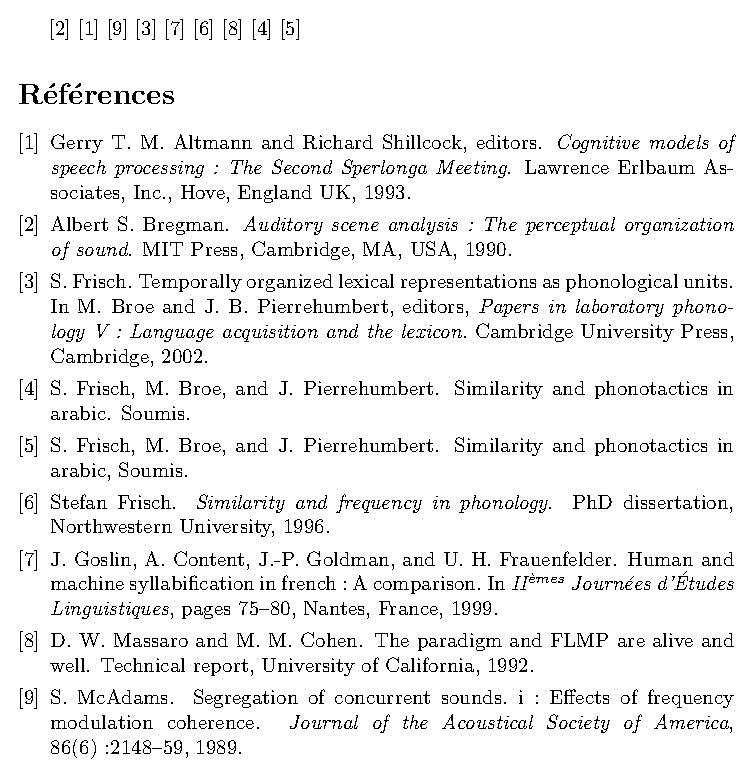
\includegraphics[width=.6\textwidth]{material/plain}
\end{center}

\section{Style \emph{unsrt}}
{\large\verb1\bibliographystyle{unsrt}1}
\begin{center}
  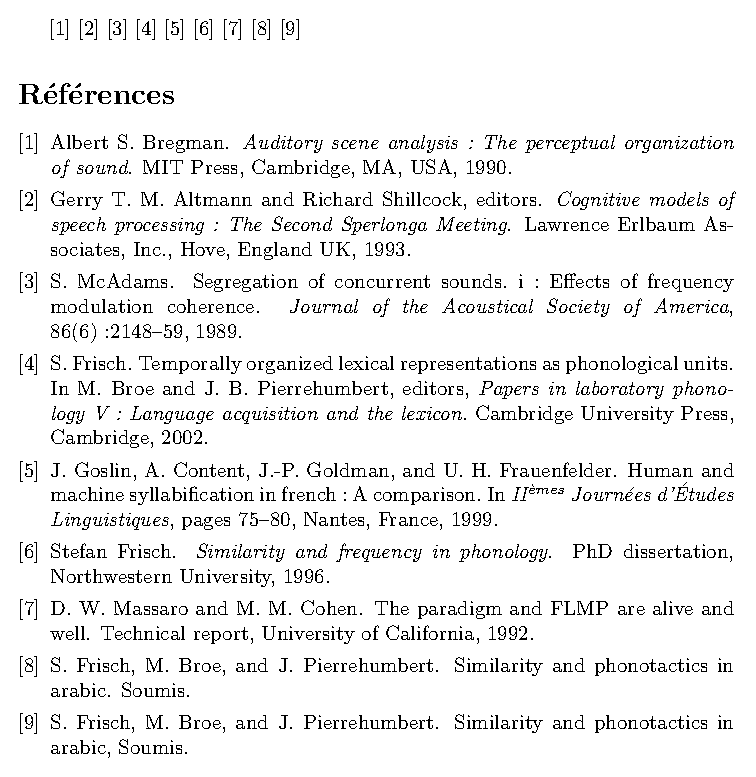
\includegraphics[width=.6\textwidth]{material/unsrt}
\end{center}

\section{Style \emph{abbrv}}
{\large\verb1\bibliographystyle{abbrv}1}
\begin{center}
  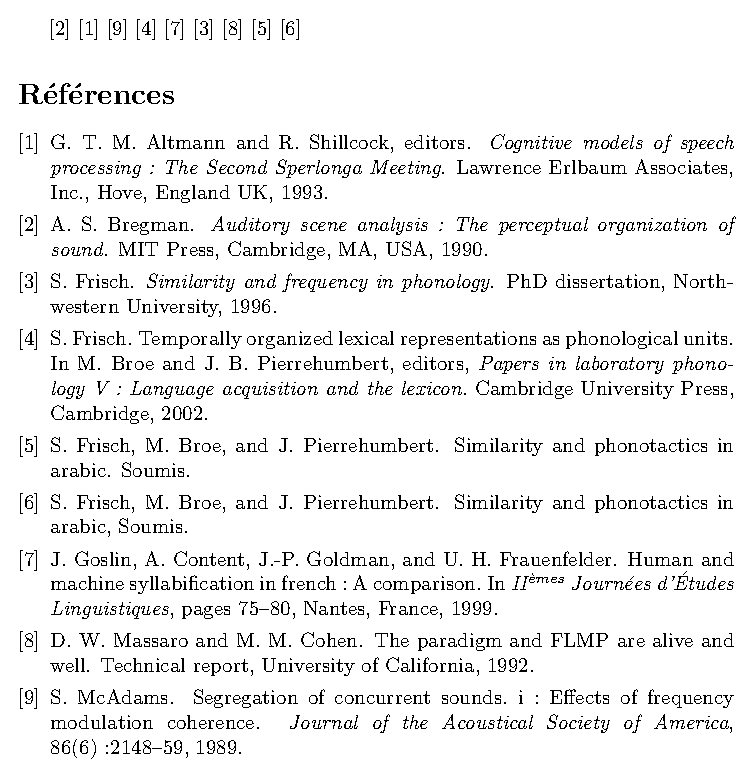
\includegraphics[width=.6\textwidth]{material/abbrv}
\end{center}

\section{Style \emph{ieeetr}}
{\large\verb1\bibliographystyle{ieeetr}1}
\begin{center}
  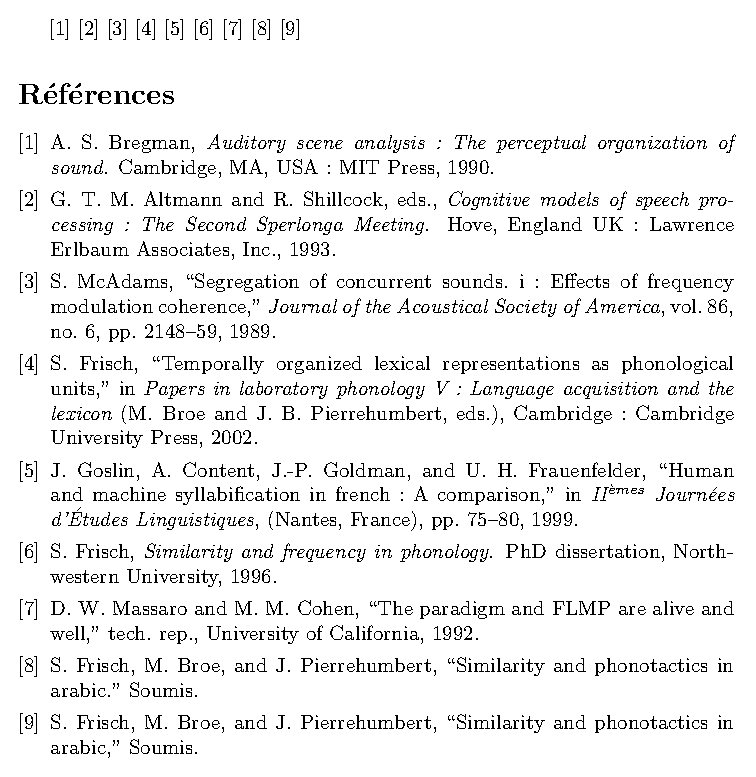
\includegraphics[width=.6\textwidth]{material/ieeetr}
\end{center}

\section{Style \emph{alpha}}
{\large\verb1\bibliographystyle{alpha}1}
\begin{center}
  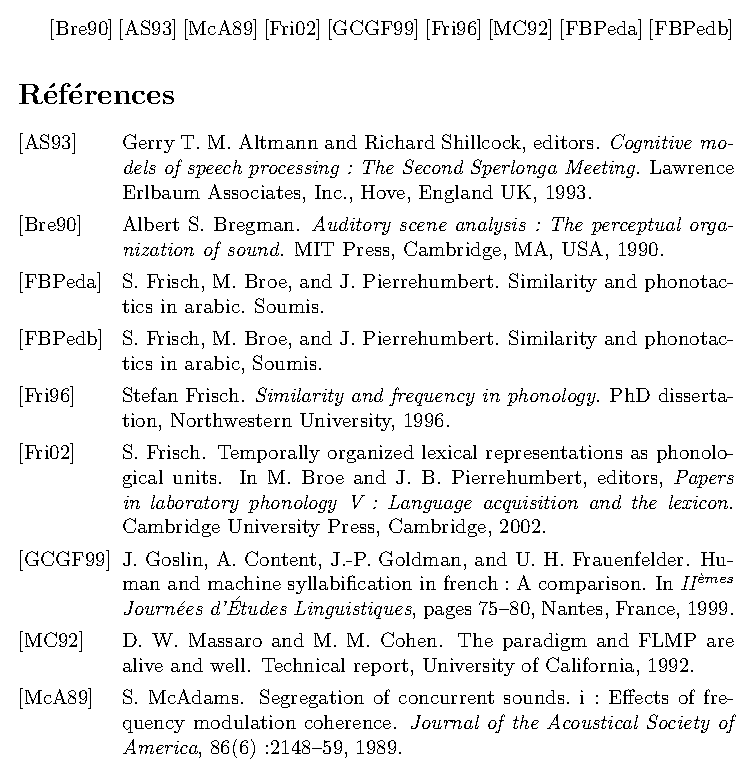
\includegraphics[width=.6\textwidth]{material/alpha}
\end{center}

\section{Style \emph{siam}}
{\large\verb1\bibliographystyle{siam}1}
\begin{center}
  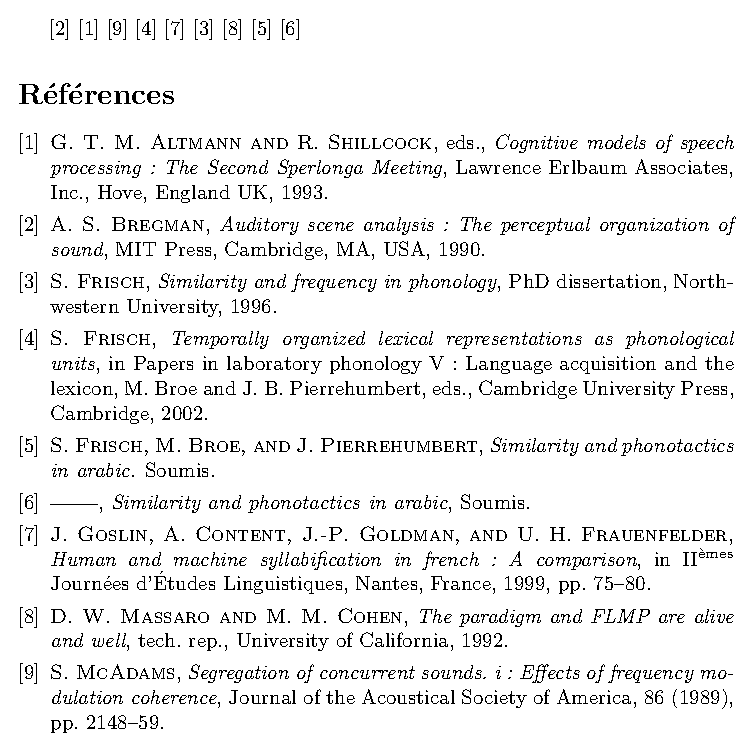
\includegraphics[width=.6\textwidth]{material/siam}
\end{center}

\section{\ldots et en utilisant l'extension \emph{natbib}}
\begin{center}
  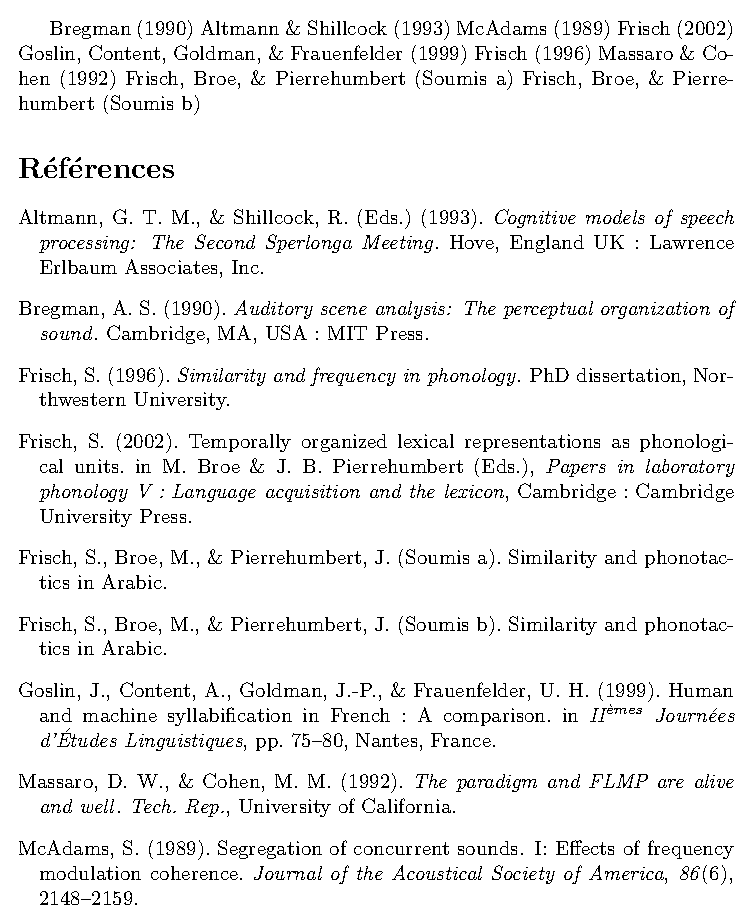
\includegraphics[width=.5\textwidth]{material/natbib-apaformat}
\end{center}





\section{Utilisation de BIB\TeX\  avec \LaTeX}
\pagecolor{\BGColor}
\color{\FGColor}

\vfill
\begin{itemize}
\item Lors de la rédaction du texte, on cite les références bibliographiques en
  désignant l'entrée correspondante dans la base de données bibliographique par
  l'instruction \verb1\cite{clé-de-la-référence}1.
\item La liste des références bibliographiques, sera construite automatiquement
  à la fin du document.
\item On utilise 2 instructions pour contrôler la gestion des références
  bibliographiques :
  \begin{itemize}
  \item \verb1\bibliography{nom-de-fichier}1 indique le nom du fichier contenant
    la base de données bibliographique.
  \item \verb1\bibliographystyle{nom-du-style}1 spécifie l'apparence des appels
    et des références. Les styles \emph{standard} sont :
    \begin{itemize}
    \item plain : [1] Noam Chomsky\ldots
    \item unsrt : idem mais dans l'ordre d'apparition des appels de citation.
    \item abbrv : [1] N. Chomsky\ldots
    \item ieetr : idem mais dans l'ordre d'apparition des appels de citation.
    \item alpha : [Cho68] Noam Chomsky\ldots
    \end{itemize}
  \end{itemize}
\end{itemize}
\vfill




\section{Compilation d'un document}
\label{sec:compilation-bibtex}


\vfill
\begin{itemize}
\item \verb1$ latex1
\item \verb1$ bibtex1
\item \verb1$ latex1
\item \verb1$ latex1
\end{itemize}
\vfill




\section{Exercices}
\label{sec:exercices}
\vfill
\begin{itemize}
\item Créez votre propre base de données bibliographique.
\item Créez un document dans lequel vous allez citer ces références en
  utilisant les techniques précédentes et en choisissant un style
  (plain, alpha, ieeetr\ldots). Nous verrons l'usage de natbib plus
  tard (c'est une extension, pas un style bibliographique).
\item Compilez votre document.
\end{itemize}
\vfill








\chapter{L'extension Ref\TeX\ d'Emacs}
\label{cha:reftex}
\begin{center}
  \begin{minipage}[r]{0.5\linewidth}
    L'extension REF\TeX\ d'Emacs permet de gérer plus facilement le
    processus de citations bibliographiques et de renvois vers les
    parties du document.
  \end{minipage}
\end{center}

\section{Présentation de REF\TeX}
\label{sec:reftex}

\vfill
\begin{itemize}
\item REF\TeX\ est un mode \emph{mineur} d'Emacs qui peut s'ajouter à AUC\TeX.
\item Il a pour fonction de gérer les références de tout type\ldots et notamment
  les références bibliographiques.
\item Pour le lancer, on tape \verb1M-x reftex-mode1 dans Emacs.
\item Mais on peut aussi le charger automatiquement dès qu'AUC\TeX\ est lui-même
  lancé. Pour celà, il faut entrer les lignes suivantes dans le fichier de
  démarrage d'Emacs (\verb1.emacs1):
  \begin{itemize}
%  \item \verb1(require 'tex-site)1
  \item \verb1(add-hook 'LaTeX-mode-hook 'turn-on-reftex)1
  \item \verb1(setq reftex-plug-into-AUCTeX t)1
  \end{itemize}
\end{itemize}
\vfill

% '(reftex-default-bibliography (quote ("/home/olivier/texmf/bibtex/bib/olivier-perso.bib" "/home/olivier/texmf/bibtex/bib/speech-science.bib")))

Si le mode REF\TeX\ est bien lancé, vous devriez voir un menu \og Ref
\fg apparaître dans la barre de menu d'Emacs.

\section{Gestion des références bibliographiques}

Le menu Ref $\Rightarrow$ Cite vous permet de faire une recherche dans
votre base de données bibliographique.

Si vous sélectionnez une entrée dans celles proposées, il insère la
commande nécessaire à l'endroit où se trouve le curseur.


\section{Gestion des renvois}

La gestion des renvois fonctionne de la même manière : vous pouvez
utiliser Ref $\Rightarrow$ Label pour insérer un label, et Ref
$\Rightarrow$ Ref pour insérer un renvoi. Dans ce dernier cas, Emacs
vous proposera de sélectionner le type de référence (section,
équation, figure, tableau\ldots --un appui sur la barre espace fera
une recherche sur toutes les sources possible), puis vous présentera
une liste des éléments vers lesquels vous pouvez produire un renvoi.



\chapter{Utilisation de l'extension \texttt{natbib}}
\label{cha:natbib}
\begin{center}
  \begin{minipage}[r]{0.5\linewidth}
    L'extension \LaTeX\ \emph{natbib} est une extension
    bibliographique qui permet de produire des bibliographies et des
    appels bibliographiques conformes à certaines exigences n'ayant
    pas été prévues en standard. On retrouve ce type de \og standard
    \fg dans les sciences de la vie mais aussi dans certains
    (sous-)domaines des sciences humaines et sociales (certaines
    branches de la psychologie, de la linguistique, de la sociologie,
    de la géographie\ldots)
  \end{minipage}
\end{center}

\section{En-tête du document}

L'extension \emph{natbib} permet de générer des références
bibliographiques de type \emph{auteur (année)}. Pour utiliser
l'extension \emph{natbib}, vous appelerez cette extension dans
l'en-tête du document :


\begin{verbatim}
\usepackage[longnamesfirst,round]{natbib}
\end{verbatim}

Les options (facultatives) présentées ici ont pour fonction (1) de
forcer l'affichage de la liste intégrale des auteurs au premier appel
et (2) de présenter l'année de publication entre parenthèses.







\section{Appel des références bibliographiques}

Afin d'utiliser au mieux l'extension natbib, il convient de prendre
l'habitude d'utiliser différentes formes de \verb1\cite1 afin de
contrôler précisément le type de renvoi bibliographique :


\begin{itemize}
\item \verb1\cite{} = \citet{}1 (c'est la forme par défaut, cite le
  nom d'auteur(s) \emph{dans le texte} et affiche l'année entre
  parenthèses);

\item \verb1\citep{}1 (tout entre parenthèses, une virgule sépare la
  liste des auteurs de l'année);

\item \verb1\citeauthor{}1 (auteur seul);

\item \verb1\citeyear{}1 (année seule);

\item \verb1\cite[chap.~2]{}1 (commentaire après la citation);

\item \verb1\cite[cf.][]{}1 (commentaire avant la citation);

\item \verb1\cite[cf.][chap.~2]{}1 (commentaires avant \emph{et} après
  la citation);

\item \verb1\cite*{}1 (force la citation de tous les auteurs au lieu
  de et al. pour cet appel, toutes les autres formes affichant les
  noms d'auteurs peuvent être suivies d'une astérisque pour produire
  le même effet).
\end{itemize}






\section{Formatage de la bibliographie}

Comme d'habitude, vous introduirez --à l'endroit où vous souhaitez
faire apparaître votre liste de références bibliographiques-- les
commandes suivantes :

\begin{verbatim}
\bibliography{nom-de-votre-base}
\bibliographystyle{abbrvnat}
\end{verbatim}

Pour le reste, le fonctionnement est similaire. L'extension
\emph{natbib} fournit des formats de bibliographies permettant de
remplacer les formats standards (les noms sont similaires mais se
terminent par -nat).

Vous pouvez aussi utiliser le format \verb1apaformat.bst1 que je tiens
à votre disposition et qui reproduit des exigences communes dans de
nombreux sous-domaines des sciences humaines et sociales (type
\emph{American Psychological Association}).


%%% Local Variables: 
%%% mode: latex
%%% TeX-master: "~/home/teaching/cours/sdl/M2/LaTeX/slides/recueil-initiation-LaTeX"
%%% End: 



 \chapter{Utilisation de l'extension \texttt{jurabib}}
 \label{cha:jurabib}
 \begin{center}
   \begin{minipage}[r]{0.5\linewidth}
     L'extension \LaTeX\ \emph{natbib} est une extension
     bibliographique qui permet de produire des bibliographies et des
     appels bibliographiques conformes à certaines exigences n'ayant
     pas été prévues en standard. On retrouve ce type de \og standard
     \fg en littérature et dans certains (sous-)domaines des sciences
     humaines et sociales (psychologie, linguistique, philosophie,
     histoire\ldots).

   \end{minipage}
 \end{center}

 
\section{Les objectifs de \emph{jurabib}}


L'extension jurabib permet notamment de gérer des systèmes
bibliographiques requérant une présentation des références
bibliographiques en notes de bas de page, laquelle est assortie de
termes particuliers lorsque la référence a déjà été citée (op. cit.,
idem, ibidem\ldots).

L'atout majeur de jurabib est qu'il vous permettra de respecter toutes
ces règles \emph{sans avoir besoin de savoir (1) si vous avez déjà
  cité une référence, (2) quel terme vous devez utiliser si la
  référence a déjà été citée\ldots)}


\section{En-tête du document}

Pour utiliser \emph{jurabib} on charge l'extension et on définit un
certain nombre de paramètres :


\begin{small}
\begin{verbatim}
\usepackage{jurabib}
\jurabibsetup{%
  human=true,
  authorformat={abbrv,and,year,smallcaps},
  bibformat={ibidem},
  commabeforerest,
  ibidem=strict,
  idem=strict,
  opcit=true,
  citefull=first,
  biblikecite=true,
  oxford=true,
  titleformat={italic,commasep},
  annote=off,
}

\renewcommand{\bibauthormultiple}{--------\hspace{1em}}
\renewcommand{\cite}{\footcite}
\renewcommand{\bibbtsep}{in }
\renewcommand{\bibjtsep}{}
\renewcommand{\bibansep}{,}
\renewcommand{\bibatsep}{,}
\renewcommand{\bibbdsep}{}
\renewcommand{\bpubaddr}{~:}
\renewcommand{\bibjtfont}{\textit}
\end{verbatim}
\end{small}



\section{Appel des références bibliographiques}

Le fonctionnement est ensuite proche de celui de \emph{natbib} pour
les appels bibliographiques :


\begin{verbatim}

\cite{}
\citeauthor{}
\citeyear{}
\cite[p.15]{}

\end{verbatim}




\section{Formatage de la bibliographie}

Tout comme avec les autres systèmes, on indique le nom de la base
bibliographique et le style bibliographique (utilisez \emph{jox} qui
est fourni avec jurabib).

Si vous ne souhaitez pas qu'une bibliographie finale soit insérée dans
votre document, vous remplacerez \verb1\bibliography{}1 par
\verb1\nobibliography{}1.


\begin{verbatim}
\bibliography{filename} (ou \nobibliography{filename})
\bibliographystyle{jox}
\end{verbatim}


%%% Local Variables: 
%%% mode: latex
%%% TeX-master: "~/home/teaching/cours/sdl/M2/LaTeX/slides/recueil-initiation-LaTeX"
%%% End: 



\chapter{Personnalisation de la mise en page}
\label{cha:personnalisation}
\begin{center}
  \begin{minipage}[r]{0.5\linewidth}
    Ce chapitre vous permettra de mieux comprendre comment on peut
    influencer la mise en page prévue en standard par
    \LaTeX. Modification des formats de page, des marges, des
    paragraphes, des titres de section, en-têtes et pieds de
    page\ldots
  \end{minipage}
\end{center}


\section{Le contrôle des tailles avec \LaTeX}

Dans les pages suivantes, un certain nombre de commandes contrôlent
des dimensions qui prises en compte par \LaTeX\ lors du formatage. Les
dimensions peuvent être exprimées dans différentes unités, parmi
lesquelles :

Les quatre premières unités (cm, mm, in, pt) sont des unités absolues
(leur valeur reste la même quel que soit le contexte dans lequel on se
trouve). Les deux dernières sont des unités dites relatives (leur
valeur réelle dépend du contexte, c'est à dire de la taille de la
police en cours).


\begin{description}
\item[cm] centimètres;
\item[mm] millimètres;
\item[in] pouces (inches);
\item[pt] points (dimension informatique);
\item[ex] taille verticale d'un \emph{x} (permet d'indiquer une taille
  relative à la police utilisée);
\item[em] taille horizontale d'un \emph{m} (permet également
  d'indiquer une taille relative à la police utilisée);
\end{description}

\section{Double interligne}

Dans la plupart des documents universitaires (mais aussi parfois lors
de la soumission d'articles dans des revues scientifiques), il vous
est demandé de fournir des textes avec une interligne double. Il
existe une extension destinée spécifiquement à cet usage :

\begin{verbatim}
\usepackage{setspace}
\doublespacing

ou

\onehalfspacing

\end{verbatim}

Comme d'habitude, l'appel de l'extension se fait dans l'en-tête du
document.

La commande \verb1\doublespacing1 (ou \verb1\onehalfspacing1) est
aussi introduite dans l'en-tête; elle est valable pour l'ensemble du
document.

A priori, vous \emph{ne devez pas} changer ce paramètre en cours de
document. Si toutefois vous tenez absolument à le faire, l'extension
fournit aussi des environnement permettant de changer temporairement
le réglage.


\section{Marges}

L'extension \emph{geometry} permet de contrôler précisément la taille
des marges du document (entre autres). Son utilisation est très simple
:

\begin{verbatim}
\usepackage[left=5cm,right=4cm,bottom=2.5cm,top=2.5cm]{geometry}
\end{verbatim}






\section{Formatage de la page de titre}

Pour formater votre page de titre, vous pouvez, à la place de
l'instruction \verb1\maketitle1 vue au début du cours, utiliser un
code similaire à ce qui suit et l'adapter à votre convenance :


\begin{footnotesize}
\begin{verbatim}
\begin{titlepage}
  \singlespacing
  \sffamily
  \begin{center}
    {\bfseries\large Université de Nantes}\\
    {UFR Lettres et Langages}\\
    {Année Universitaire 2005--2006}\\
    \vfill

    {\Large\bfseries Titre du Mémoire}

    \vspace{2ex} {\large \'Eventuellement un sous-titre}
     
    \vspace{8ex}
    Prénom Nom\\
    Date

    \begin{flushright}
      \vfill
      \begin{tabular}{lr}
        Membres du Jury : & \\
        & Nom, Prénom (directeur du mémoire)\\
        & Nom, prénom\\
      \end{tabular}
    \end{flushright}
    \vspace{8ex}
    
    { Master 2 mention \og Langues et Langages \fg\\
      Spécialité \og Sciences du Langage \fg\\
    Parcours \og Informatisation des Langues \fg\\}
  \end{center}
\end{titlepage}
\end{verbatim}
\end{footnotesize}




\section{En-têtes et Pieds de pages}

Pour contrôler les en-têtes et les pieds de page, on utilise
l'extension \emph{fancyhdr} (pour \emph{fancy headers}). On déclare
que le style de page utilisé sera le style \emph{fancy} (celui produit
par cette extension) et on définit la nature des différentes parties
de ces éléments.

On définit ci-dessous les caractéristiques de l'en-tête droite et
gauche et celles du pied de page au centre (dans lequel on va placer
les numéros de page).

On met ensuite la largeur des lignes de séparation entre l'en-tête et
le texte (et respectivement le pied de page) à 0 points (pas de
lignes).

Les commandes \verb1\rightmark1 et \verb1\leftmark1 permettent de
faire varier le texte de manière automatique (en fonction des classes
de documents, les en-têtes gauche et droit contiendront par exemple
les noms des auteurs, le titre du document, le titre du chapitre en
cours\ldots

\begin{verbatim}
\usepackage{fancyhdr}
\pagestyle{fancy}

\fancyhf{} % ici, on vide les en-têtes et pieds de page avant de les définir

\fancyhead[R]{\small \sffamily En-tête à droite} (on peut par exemple mettre \rightmark)
\fancyhead[L]{\small \sffamily En-tête à gauche} (on peut par exemple mettre \leftmark)
\fancyfoot[C]{\small \sffamily \thepage}
\renewcommand{\headrulewidth}{0pt}
\renewcommand{\footrulewidth}{0pt}
\end{verbatim}


\section{Personnalisation des titres de section (mode de numérotation)}

On contrôle le mode de numérotation en redéfinissant les commandes
suivantes (qui sont utilisées automatiquement par \LaTeX\ lors de la
compilation). Il convient, au préalable, de \emph{relever} la
profondeur de section au-delà de laquelle s'interrompt la numérotation
des sections.

{\small
\begin{verbatim}
\setcounter{secnumdepth}{7}

\def\thechapter{\Roman{chapter}}
\def\thesection{\Alph{section}}
\def\thesubsection{\Roman{subsection}}
\def\thesubsubsection{\arabic{subsubsection}}
\def\theparagraph{\roman{paragraph}}
\def\thesubparagraph{\alph{subparagraph}}
\end{verbatim}
}

\section{Personnalisation des titres de section (changement de mise en forme simple)}

On fait appel à l'extension \emph{sectsty} et on redéfinit chaque
niveau de section (alignement du texte, taille de la police, graisse,
type de police, éventuellement suppression de la numérotation des
pages, insertion d'un saut de page préalable).

{\small
\begin{verbatim}
\usepackage{sectsty}

%\partfont{\centering\Huge\bfseries\sffamily\thispagestyle{empty}}
%\chapterfont{\Large\bfseries\sffamily}
\sectionfont{\newpage\raggedleft\large\bfseries\sffamily}
\subsectionfont{\large\mdseries\sffamily}
\subsubsectionfont{\normalsize\mdseries\sffamily}
\end{verbatim}
}


\section{Personnalisation des titres de section (changement de mise en forme plus complexe)}

On fait appel à l'extension \emph{titlesec} (et ici on ajoute un
recours à l'extension \emph{scalefont} qui permet de gérer plus
finement les tailles de police). Le format des commandes est le suivant :

{\small
\begin{verbatim}
\titleformat{niveau}[formatage du paragraph]{formatage du titre}{formatage du numéro}...
                          ...{espacement entre numéro et titre}{code à insérer après le titre}
\end{verbatim}
}

{\scriptsize
\begin{verbatim}
\usepackage{scalefnt}
\usepackage{titlesec}

\titleformat{\part}[display]{\raggedleft\Huge\scalefont{1.3}\sffamily\bfseries\thispagestyle{empty}}{\partname}{0cm}{}
\titleformat{\chapter}[display]{\raggedleft\Huge\sffamily\bfseries}{\chaptertitlename\ \thechapter}{0cm}{}
\titleformat{\section}{\Large\sffamily\bfseries}{\thesection)\quad}{0cm}{}
\titleformat{\subsection}{\Large\sffamily}{\thesubsection --\quad}{0cm}{}
\titleformat{\subsubsection}{\large\sffamily\itshape\raggedright}{\thesubsubsection.\quad}{0cm}{}
\titleformat{\paragraph}{\normalsize\sffamily\itshape\raggedright}{\theparagraph\quad}{0cm}{}
\titleformat{\subparagraph}{\normalsize\sffamily\itshape\raggedright}{\thesubparagraph\quad}{0cm}{}
\end{verbatim}
}


\section{Modification des paragraphes}

On peut modifier très simplement l'indentation par défaut (espace en
début de ligne lors des changements de paragraphe) et l'espacement
vertical entre paragraphes :

\begin{verbatim}
\setlength{\parindent}{0cm}
\setlength{\parskip}{1em}
\end{verbatim}



\section{Et maintenant ?}

Si vous avez réussi à tenir jusqu'au bout, alors vous êtes sur la
bonne voie\ldots mais votre apprentissage est loin d'être fini. Il
existe très certainement un millier de choses que vous souhaiteriez
pouvoir faire sans encore savoir comment vous pourriez vous y prendre
avec \LaTeX. Il vous faudra faire preuve de beaucoup de patience et
d'un travail régulier, lire la documentation qui fourmille sur
internet, vous procurer un livre (éventuellement en format
électronique, cf. les références données p.~\pageref{sec:freebooks}),
rechercher des extensions qui pourraient répondre à vos besoins en
consultant le \emph{Comprehensive Tex Archive Network}
(p.~\pageref{sec:websites}).

N'hésitez pas aussi à rechercher la réponse à vos problèmes dans les
foires aux question (p.~\pageref{sec:faq}) et à consulter
régulièrement les \emph{newsgroups} (p.~\pageref{sec:newsgroups}).

\vfill

\hfill Bon courage\ldots et bonne route avec \LaTeX !

\vfill


% double interligne
% geometry
% formatage page de titre (standard Université)
              




% \chapter{L'indexation des documents}
% 


\section{Les bases de l'indexation}


\verb1\usepackage{index}1

\verb1\proofmodetrue1

\verb1\newindex{default}{idx}{ind}{Index des notions}1 ou \verb1\makeindex1

\verb1\newindex{aut}{adx}{and}{Index des auteurs}1

\begin{verbatim}
  latex file.tex
  makeindex (= makeindex -o file.ind file.idx)
  makeindex -o file.and file.adx
  latex file.tex

  latex file.tex && makeindex file.idx && latex file.tex
\end{verbatim}

\verb1\makeindex1 (dans le préambule du document)

mot à indexer\verb1\index{mot à indexer}1

ou

\verb1\index{mot à indexer}1mot à indexer (pas d'espace au cas où un saut de
page venait séparer le mot de son indexation.)

ou

\verb1\index*{mot à index}1



\verb1\printindex1 à l'endroit où l'on souhaite faire apparaître l'index.







%%% Local Variables: 
%%% mode: latex
%%% TeX-master: "recueil-initiation-LaTeX"
%%% End: 



% \chapter{Recherche et Installation d'extensions supplémentaires}
% \section{Installation d'une extension sous windows}

\vfill
\begin{itemize}
\item Aller sur CTAN (http://www.ctan.org) ou l'un de ses mirroirs.
\item Télécharger l'archive correspondant à l'extension
\item Extraire l'archive dans c:$\backslash$Program
  Files$\backslash$TeXLive$\backslash$texmf-local$\backslash$
\item Démarrer -> Prgrammes -> Accessoires -> Invite de commande
\item cd C:$\backslash$Program Files$\backslash$TeXLive$\backslash$texmf-local$\backslash$extension$\backslash$
\item latex extension.ins
\item latex extension.dtx
\item Démarrer -> Programmes -> TeXLive -> Maintenance -> Rebuild ls-R filenames databases
\item Utiliser l'extension.
\end{itemize}
\vfill



% \chapter{Questions et problèmes divers}
% \include{inputs/misc-LaTeX}


% \chapter{Outils pour la linguistique}
% \include{inputs/linguistique.tex}


\listoffigures
\label{list:fig}

\listoftables
\label{list:tab}

%\listof{exemple}{Liste des exemples}

%\newpage
% \vspace*{4cm}
% \begin{center}
% \large Ce document peut-être téléchargé sur le site :\\
% \url{http://www.lettres.univ-nantes.fr/sdl/teaching/master/latex/}  
% \end{center}
% \vfill


%%% Local Variables: 
%%% mode: latex
%%% TeX-master: "ED-Initiation-LaTeX-couleur"
%%% End: 



\end{document}




%% Installation d'une extension sous windows :

%% Aller sur CTAN
%% Télécharger l'archive correspondant à l'extension
%% Extraire l'archive dans c:\Program Files\TeXLive\texmf-local\

%% Démarrer -> Prgrammes -> Accessoires -> Invite de commande

%% cd C:\Program Files\TeXLive\texmf-local\extension\

%% latex extension.ins
%% latex extension.dtx

%% Démarrer -> Programmes -> TeXLive -> Maintenance -> Rebuild ls-R filenames databases

%% Utiliser l'extension.








%%% Local Variables: 
%%% mode: latex
%%% TeX-master: "recueil-initiation-LaTeX"
%%% End: 
